%%%%
%%%% Multiagent Simulation and the MASON Library
%%%% GeoMason GIS extension
%%%%
%%%% Copyright 2012 by Mark Coletti
%%%%
%%%% LaTeX Source
%%%% This source code, and embedded PDFs and sources (such as OmniGraffle Files)
%%%% Are distributed under the Academic Free License version 3.0
%%%% See the file "LICENSE" for more information
%%%%
%%%% When you build this source code, the resulting PDF file is licensed under the
%%%% Creative Commons Attribution-No Derivative Works 3.0 United States License
%%%% See the URL http://creativecommons.org/licenses/by-nd/3.0/us/   for more information
%%%%
%%%% If you have any questions, feel free to contact me at mcoletti@gmail.com

\documentclass[twoside,10pt]{book}
\usepackage{fullpage}
\usepackage{mathpazo}
%\usepackage[noend]{algpseudocode}
\usepackage{amsmath}
\usepackage{latexsym}
\usepackage{graphicx}
\usepackage{wrapfig}
\usepackage{bm}
%\usepackage{qtree}
\usepackage{array}
\usepackage{eurosym}
\usepackage{textcomp}
\usepackage{makeidx}
\usepackage{rotating}
\usepackage{multirow}
\usepackage{multicol}
\usepackage{microtype}
\usepackage{afterpage}
\usepackage{color}\definecolor{gray}{gray}{0.5}
\usepackage{xcolor}
\usepackage{alltt}
\usepackage{fancyvrb}
\usepackage[font=footnotesize,labelsep=quad,labelfont=it]{caption}
%%% Added in order to use hyperref -- this stuff has to appear before bibentry,x
%%% which has a conflict with regard to \bibitem.  See later in this file for more stuff that has
%%% to be added afterwards
  \makeatletter
  \let\saved@bibitem\@bibitem
  \makeatother

\usepackage{bibentry}
\usepackage[hyperfootnotes=false,linktocpage=true,linkbordercolor={0.5 0 0}]{hyperref}
%%% Note that to avoid a link being created from \pageref, just use \pageref*
%%% End hyperref stuff

\renewcommand\textfraction{0.0}
\renewcommand\topfraction{1.0}
\renewcommand\bottomfraction{1.0}

\makeindex

\newcommand\file[1]{\textsf{#1}}
\newcommand\variable[1]{\textsf{#1}}
%\newcommand\package[1]{\textsf{#1}}
\newcommand\package[1]{\index{Packages!{#1}}\textsf{#1}}
\newcommand\Package[1]{\index{Packages!{#1}|textbf}\textsf{#1}}
%\newcommand\class[1]{\textsf{#1}}
\newcommand\class[1]{\index{Classes!{#1}}\textsf{#1}}
\newcommand\Class[1]{\index{Classes!{#1}|textbf}\textsf{#1}}
\newcommand\method[1]{\textsf{#1}}
\newcommand\member[1]{\textsf{#1}}
\newcommand\parameter[1]{\texttt{#1}}
\newcommand\character[1]{\texttt{"{#1}"}}
\newcommand\textstr[1]{\texttt{"{#1}"}}
\newcommand\code[1]{\textsf{#1}}
%\newcommand\code[1]{\texttt{#1}}

\newcommand\ignore[1]{}


\newcommand\JTS{\index{JTS Topology Suite}JTS Topology Suite }
\newcommand\JTSshort{\index{JTS Topology Suite}JTS }

\newcommand\sidebara[3]{\begin{wrapfigure}{r}[0in]{3.2in}%
\vspace{-1.1em}\hfill\framebox{\begin{minipage}{3in}\setlength\parindent{1.5em}\footnotesize{\noindent\textit{#1}

\vspace{0.5em}{\noindent #2}}
\end{minipage}}
\vspace{#3}
\end{wrapfigure}
}

\newcommand\sidebar[2]{\begin{wrapfigure}{r}[0in]{3.2in}%
\vspace{-1.1em}\hfill\framebox{\begin{minipage}{3in}\setlength\parindent{1.5em}\footnotesize{\noindent\textit{#1}

\vspace{0.5em}{\noindent #2}}
\end{minipage}}
\vspace{-0.5em}
\end{wrapfigure}
}



%%% Hack to allow more spacing before and after an hline
\newcommand\tstrut{\rule{0pt}{2.4ex}}
\newcommand\bstrut{\rule[-1.0ex]{0pt}{0pt}}

% Increase the numbering depth
\setcounter{secnumdepth}{3}
\setcounter{tocdepth}{6}


%%%% This code is used to create consistent lists of methods

% From TUGboat, Volume 24 (2003), No. 2 "Hints & Tricks"
\newcommand*{\xfill}[1][0pt]{%
	\cleaders
		\hbox to 1pt{\hss
			\raisebox{#1}{\rule{1.2pt}{0.4pt}}%
			\hss}\hfill}
			
\newenvironment{methods}[1]{
\vspace{1.0em}\noindent\textsf{\textbf{#1 Methods}}\quad \xfill[0.5ex]
\vspace{-0.25em}
\begin{description}
\small}
{\end{description}\hrule\vspace{1.5em}}

\newcommand{\mthd}[1]{\item[{\sf #1}]~\newline}


\newcommand\reference[1]{\vspace{0.5em}\hfill{\parbox{6in}{\raggedleft\noindent\textsf{#1}}}}

% Include subsubsection in the TOC
\setcounter{tocdepth}{3}

% Use with a %, like this:   \params{%
\newcommand\params[1]{\vbox{\begin{quote}\small\tt{\noindent{#1}}\end{quote}}}
\newcommand\script[1]{\params{#1}}
\newcommand\java[1]{\params{#1}}

% Allow poor horizontal spacing
\sloppy

% Allow a ragged bottom even in two-sided
\raggedbottom

% Command to push text to following page without the cutoff that occurs with clearpage
\newcommand\bump{\vspace{10in}}

% Command to push text to following line
\newcommand\hbump{\hspace{10in}}


% Define an existing word in text as an index item
\newcommand{\idx}[1]{\index{#1}#1}

% Define an existing word in text as an index item and make it bold
\newcommand{\df}[1]{\index{#1}\textbf{#1}}

% Provide a separate index item for a word in text and make it bold
\newcommand{\dfa}[2]{\index{#1}\textbf{#2}}

% Create algorithms and definitions
\newtheorem{algm}{Algorithm}
\newtheorem{defn}{Definition}

% Initial figures, pages, algorithms, and sections should be 0 :-)
\setcounter{figure}{-1}	% Mona is Figure 0
\setcounter{page}{-1}	% Start with Page 1 (the Front Page).  I'd like it to be Page 0 but it messes up twosided
\setcounter{algm}{-1}	% Start with Algorithm 0 (the Example Algorithm)
\setcounter{section}{-1}	% Start at Section 0 (the Introduction)

\thispagestyle{plain}
\thispagestyle{empty}

\newcommand\hsp[1]{{\rule{0pt}{0pt}\hspace{#1}}}
\newcommand\spc{{\rule{0pt}{0pt}~}}



\makeindex


\begin{document}

\begin{wrapfigure}{r}[2.5in]{4in}
\vspace{-1.1in}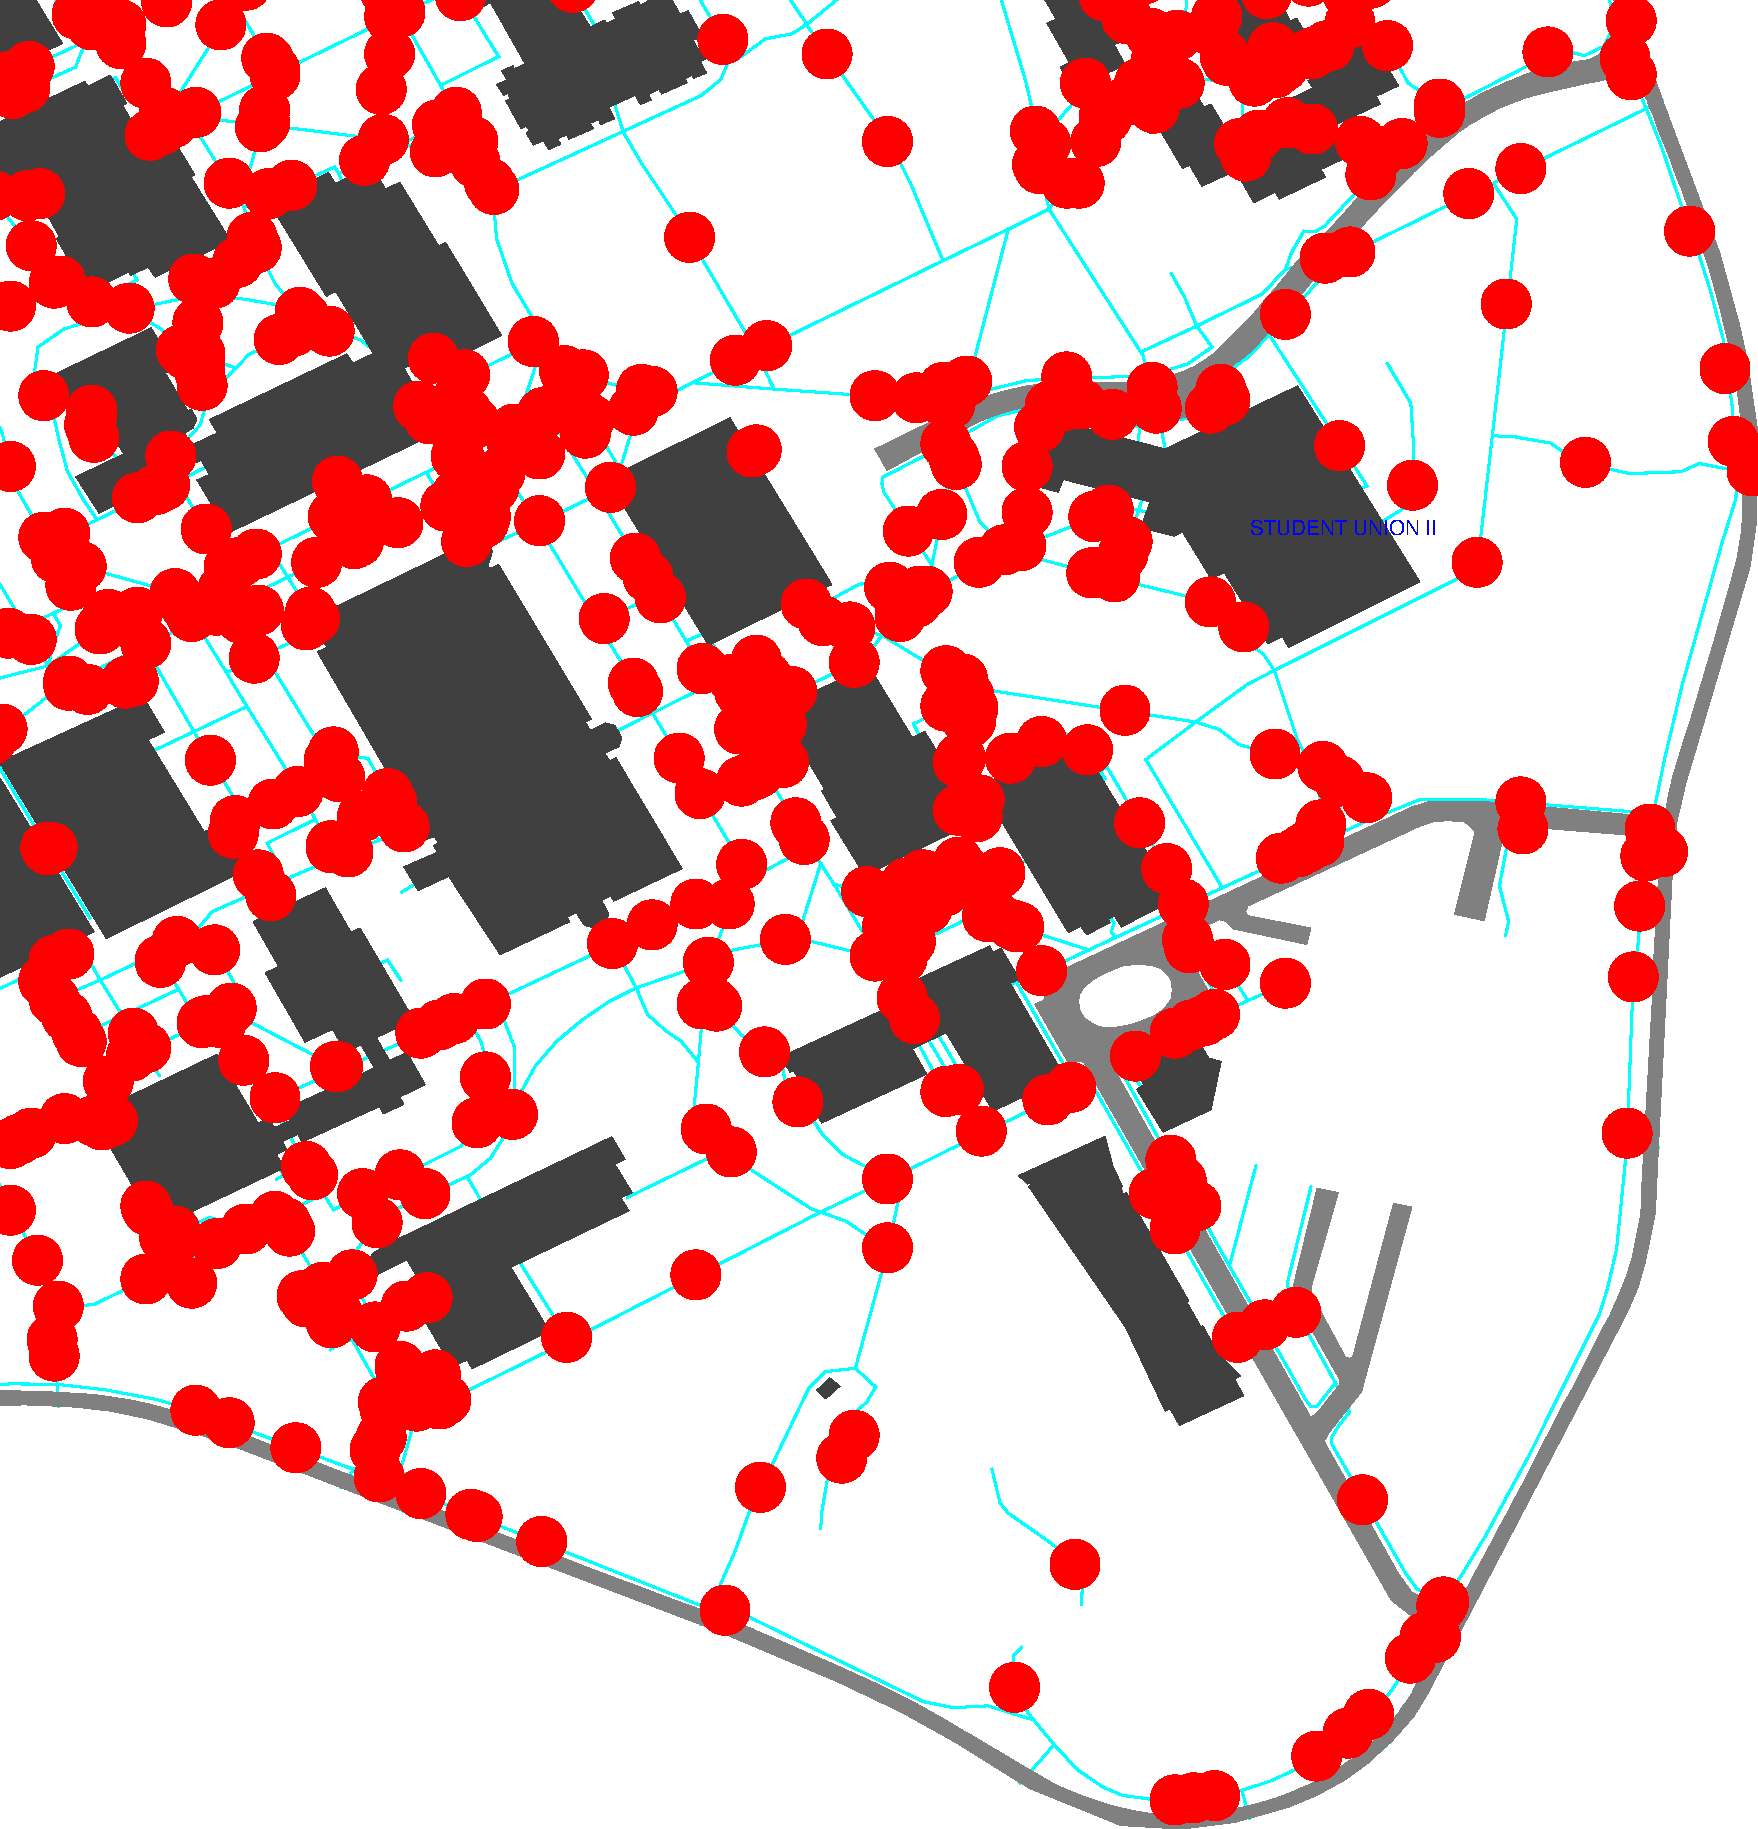
\includegraphics[height=11in]{campus.pdf}
\end{wrapfigure}

\begin{flushleft}
\huge\bf The GeoMason Cookbook\\[\baselineskip]
\end{flushleft}

\noindent\Large\bf Mark Coletti\\
{\large\rm 
Department of Computer Science\\
George Mason University}
\\
\\
\\
\Large\bf Zeroth Edition\\
\large\rm Online Version 0.1\\
\large\rm January, 2013\\

\vspace{5in}
\noindent\Large\bf Where to Obtain GeoMason\\
\large\rm http:/\!/cs.gmu.edu/\!\(\sim\)eclab/projects/mason/extensions/geomason/

\clearpage

\small 
\noindent {\Large\bf Copyright }  2012 by Mark Coletti.

\vspace{0.25in}
\noindent {\Large\bf Thanks to } Sean Luke, Andrew Crooks, Keith Sullivan

\vspace{0.25in}

\noindent {\Large\bf Get the latest version of this document or suggest improvements here:}

\reference{http:/\!/cs.gmu.edu/\!\(\sim\)eclab/projects/mason/extensions/geomason}

\vspace{0.15in}

\vspace{0.15in}
	\noindent {\Large\bf This document is licensed} under the {\bf Creative Commons Attribution-No Derivative Works 3.0 United States License,} except for those portions of the work licensed differently as described in the next section. To view a copy of this license, visit http:/\!/creativecommons.org/licenses/by-nd/3.0/us/ or send a letter to Creative Commons, 171 Second Street, Suite 300, San Francisco, California, 94105, USA.  A quick license summary:
	\begin{itemize}
	\item You are free to redistribute this document.
	\vspace{-0.5em}\item {\bf You may not} modify, transform, translate, or build upon the document except for personal use.   
	\vspace{-0.5em}\item You must maintain the author's attribution with the document at all times.
	\vspace{-0.5em}\item You may not use the attribution to imply that the author endorses you or your document use.  
	\end{itemize}
	This summary is just informational: if there is any conflict in interpretation between the summary and the actual license, the actual license always takes precedence.


\normalsize
\cleardoublepage

\tableofcontents
\clearpage


\chapter{Introduction}
\label{ch:intro}

\begin{figure}[h]\vspace{-33em}\hspace{30em}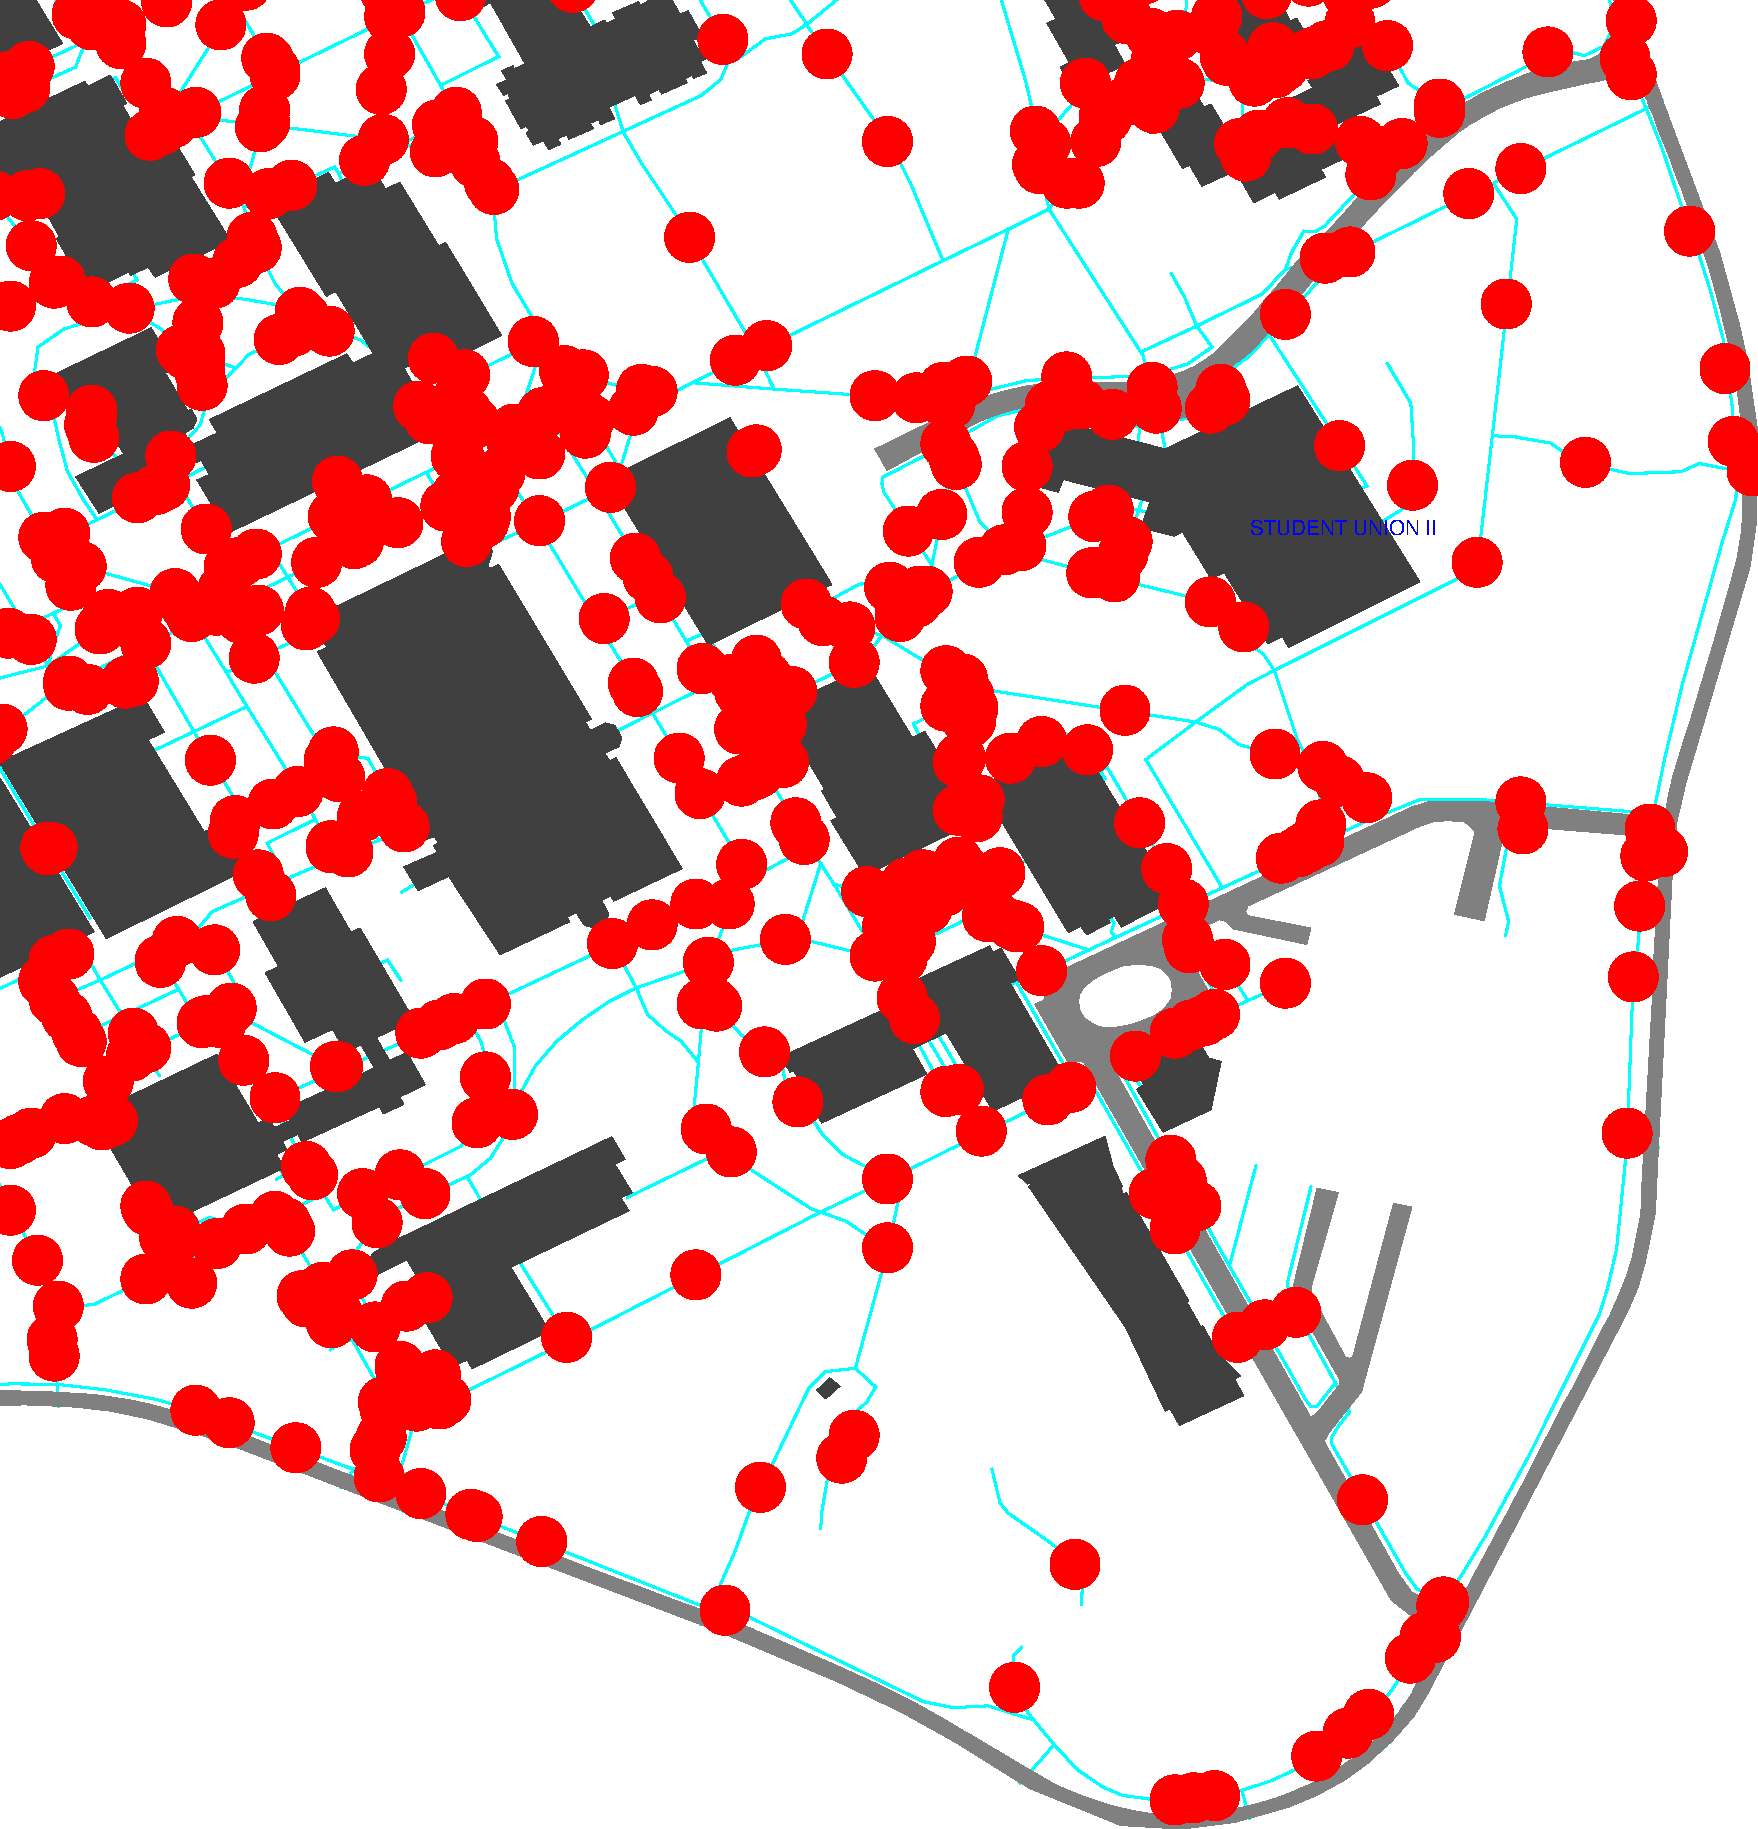
\includegraphics[width=4in]{campus.pdf}\vspace{2em}\end{figure}

%GeoMason is a MASON extension that adds basic geospatial capability.



%\begin{wrapfigure}{r}[0in]{3.7in}
%\vspace{-4em}\hfill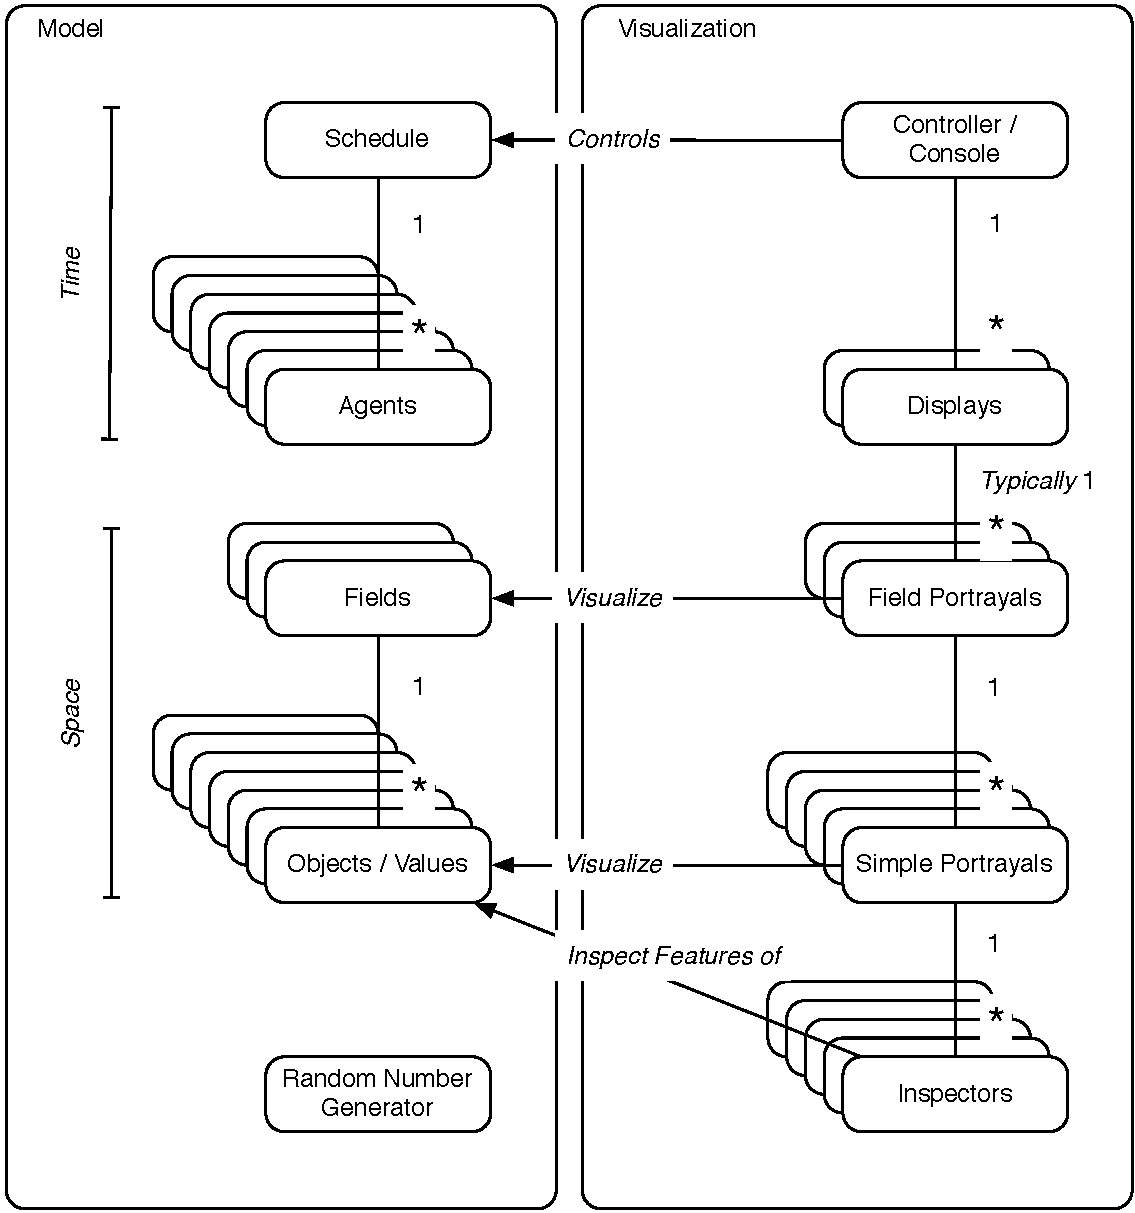
\includegraphics[width=3.7in]{MASONLayout.pdf}\vspace{-3em}\end{wrapfigure}

\section{What is GeoMason?}
MASON is a sophisticated multi-agent discrete event simulation library.
Unfortunately it does not natively support geospatial data, which
means that such support has to be hand crafted by users.  Providing
such support can be error prone and tedious to implement.

Fortunatey, there exists a MASON extension, GeoMason, that imbues
MASON with some limited geospatial awareness.  With GeoMason one is
able to load, display, and manipulate data that is, in some way,
grounded to the Earth's surface.
\section{The Motivation Behind this Book}
This ``cookbook'' provides a set of ``recipes'' for using GeoMason and is
meant to fill in the documentation gap between javadoc generated API
documentation and the GeoMason technical report.  I felt that a full
blown manual would do little more than elaborate on what was found in
the API documentation.  That is, a manual would explain the
``what'' and still leave the ``how'' largely unanswered.  The ``cookbook''
format is popular in technical literature because it provides an
accessible ``use case'' oriented style.  In the cookbook format, it's
easy for a reader to find a use case, or ``recipe,'' that best matches what
they want to do, and then use that recipe as inspiration for their own
tailored solution.  And so I felt that this format best addressed the
``how''.

For those unfamiliar with the ``Cookbook'' format, a technical
``Cookbook'' is comprised of \emph{recipes}.  Again, these recipes
embody a simple use case, and is summarized by its title such as
``Moving Agents Along a Path.''  Each recipe is comprised of a simple
problem statement, a simple solution statement optionally followed by
code examples, and then lastly followed by a discussion section that
elaborates on the problem and posed solution.

\section{What this Book Is Not}

Unfortunately I have had to make a few assumptions with this book,
which I hope are reasonable.  In particular, I presume that readers
are familiar with MASON, Geospatial Information Systems (GIS), and,
naturally, java.  This Cookbook is not intended to be a MASON, GIS, or
java primer.  If you are unfamiliar with MASON, I recommend reading
its manual
\footnote{\url{http://cs.gmu.edu/~eclab/projects/mason/manual.pdf}}
and working through its tutorials.  If you need to bone up on GIS,
there exist many resources to get you up to speed.  The Wikipedia page
for GIS is a good online starting
point.\footnote{\url{http://en.wikipedia.org/wiki/Geographic_information_system}}
The book \emph{Geographic Information Systems and Science} by
Goodchild et al is also an accessible read.\footnote{Longley, P.A.,
  Goodchild, M.F., Maguire, D.J. and Rhind, D.W. (2005) Geographic
  Information Systems and Science. Chichester: Wiley. 2nd edition.}
Naturally there exist numerous online resources on java.

\section{Book Organization}

I've divided the book into five chapters of which the first one
you're reading now.  The second chapter provides I/O related recipes;
i.e., recipes for reading and writing geospatial data using GeoMason.
The third chapter is by far the most complex --- and, even then I
confess it probably falls short of some needs.  This chapter deals
with \emph{using} GeoMason to some end, whether it's as basic as
finding nearby objects or moving agents along paths or having agents
follow gradients. I hope to in the future expand some of the leaner
recipes, particularly those involving shortest path computations, and
to add new ones, especially ones suggested by the GeoMason community.
The next chapter involves recipes for displaying geospatial data such
as rendering boundary lines over grid data.  And, finally the last
chapter has a couple recipes for common GeoMason problems; hopefully
this chapter won't expand much over time!


%%
%% Chapter 2
%%

\chapter{Reading and Writing Geospatial Data}
\label{ch:io}

This chapter covers recipes for reading and writing vector and grid based geospatial data.

\section{Reading Geospatial Data}
\label{sec:readingdata}
This section covers reading geospatial data into MASON using GeoMason.
% TODO expand this to address vector vs. raster data.  Address assumptions of GIS background of reader.

\subsection{Reading a Shape File}
\label{sub:readingshapefiles}

\begin{description}
\item[Problem] ~\\
You want to read vector geospatial data stored in a Shape
file.\index{Shape files!reading|(}

\item[Solution]~\\
Create a \class{GeomVectorField} and use \method{ShapeFileImporter.read()} to load data into it.
\begin{Verbatim}[frame=lines,framesep=5mm,commandchars=+\[\]]
// WIDTH and HEIGHT correspond to arbitrary display dimensions
private final int WIDTH = 300;
private final int HEIGHT = 300;
GeomVectorField vectorField = new GeomVectorField(WIDTH, HEIGHT);

try {
   ShapeFileImporter.read("file:foo.shp", vectorField);
} catch (FileNotFoundException ex)
{  /* handle exception */  }
\end{Verbatim}

\item[Discussion]~\\
Though there exist other GeoMason classes capable of reading Shape
files --- \class{GeoToolsImporter} and \class{OGRImporter} --- the
native GeoMason shape file importer, \class{ShapeFileImporter}, is
recommended, especially given that it has no third party dependencies
as the other importer classes do.

Given the general static nature of shape files, the above code snippet
is likely to be in a \class{SimState} subclass constructor.
Alternatively you may place it in the \method{start()} though be mindful
that means that the shape file will be loaded again each time the
simulation is restarted.

Note that the units of the loaded vector layer will be those of the
underyling coordinate reference system.  So if the shape file is
in meters, such as is found in data in Universal Transverse Mercator (UTM), then all loaded
geometry will similarly be in meters.   Also note that GeoMason uses
the \JTS to store all the geometry.  \JTS uses a
flat Cartesian plane for all points; so be aware of this when loading
data from a non-planar reference system.  That is, if you na\"{i}vely
load, say, native lat/lon data, which corresponds to coordinates along
a ellipsoid, that you will have introduced distortions in the implicit
projection you have just done to a 2D plane.  Moreover, these
distortions will be more pronounced for large surface areas.

Note that \code{WIDTH} and \code{HEIGHT} correspond to the display
dimensions and are used to help properly scale the rendered field when
panning and zooming. Note  that at some point the need for specifying
the field width and height will be unnecessary.
\end{description}



\subsection{Reading Multiple Vector Layers}
\label{sub:multiplevectorlayers}

\begin{description}
\item[Problem]~\\
You want to read in more than one thematic layer of vector
data.

\item[Solution]~\\
After ensuring that each layer uses the same coordinate reference
system, read in each layer, and then synchronize the minimum bounding
rectangles (MBR) for all the layers.\index{minimum bounding rectangle}
\begin{Verbatim}[frame=lines,framesep=5mm,commandchars=+\[\]]
GeomVectorField firstVectorField = new GeomVectorField(WIDTH,HEIGHT);
GeomVectorField secondVectorField = new GeomVectorField(WIDTH,HEIGHT);
GeomVectorField thirdVectorField = new GeomVectorField(WIDTH,HEIGHT);

try {
   ShapeFileImporter.read("file:foo.shp", firstVectorField);
   ShapeFileImporter.read("file:bar.shp", secondVectorField);
   ShapeFileImporter.read("file:baz.shp", thirdVectorField);
} catch (FileNotFoundException ex)
{  /* handle exception */  }

+color[red]Envelope globalMBR = firstVectorField.getMBR();+label[ex:MBRstart]

+color[red]globalMBR.expandToInclude(secondVectorField.getMBR());
+color[red]globalMBR.expandToInclude(thirdVectorField.getMBR());

+color[red]firstVectorField.setMBR(globalMBR);
+color[red]secondVectorField.setMBR(globalMBR);
+color[red]thirdVectorField.setMBR(globalMBR);+label[ex:MBRend]
\end{Verbatim}

\item[Discussion]~\\
It is possible that the disparate shape files may have different
coordinate reference systems, as can happen if the shape files came
from different sources.  It is vitally important to ensure that all
the layers have the same coordinate reference system before being
loaded into GeoMason.  For example, a vector layer that uses lat/lon coordinates
will have radically different geometry values from another vector layer that
uses UTM even though they may cover the same area on Earth.
Essentially, GeoMason is not a GIS so it will not do
on-the-fly projections of the data.  Users can use a real GIS tool,
such as QuantumGIS \footnote{http://www.qgis.org/}, to manually
reproject data prior to loading into GeoMason.

It is important to ensure that all the layers have the same MBR
otherwise they will not align properly when displayed.  Naturally,
this is optional if you do not intend on rendering the layers.
Regardless it would be prudent to do so anyway on the chance that
later you change your mind and want to see the
\class{GeomVectorField}s.  The highlighted lines
\ref{ex:MBRstart}-\ref{ex:MBRend} show how to synchronize the MBRs
between loaded \class{GeomVectorField}s.  Basically, you get the MBR
of the first \class{GeomVectorField}, expand it to include the area of
the MBRs for the remaining \class{GeomVectorField}s, and then set them
all to the one all-inclusive MBR.  Note that the successive calles to
\method{expandToInclude()} monotonically increase the returned MBRs.

As noted in recipe \ref{sub:readingshapefiles}, given the general
static nature of shape files, this code snippet is likely to be done
in the \class{SimState} constructor; however, again, the layers could
also be loaded via \method{start()}, though that means loading the shape
files every time the simulation is re-run.
\end{description}



\subsection{Reading a Shape File and Some of Its Attributes}
\label{sub:readingshapefileattributes}

\begin{description}
\item[Problem]~\\
You want to read a Shape file and only some of its associated
attributes.\index{Shape files!reading|)}\index{Shape files!attributes}

\item[Solution]~\\
Read in a shape file as in recipe \ref{sub:readingshapefiles}, but
specify the desired attributes by creating a \class{Bag} of \code{String}s
containing attribute names, and then passing that \class{Bag} to
\method{ShapeFileImporter.read()}.

\begin{Verbatim}[frame=lines,label=\textsf{Reading Attributes},framesep=5mm,commandchars=+\[\]]
GeomVectorField vectorField = new GeomVectorField(WIDTH,HEIGHT);

+color[red]Bag desiredAttributes = new Bag();+label[ex:attributestart]
+color[red]desiredAttributes.add("NAME");
+color[red]desiredAttributes.add("TYPE");+label[ex:attributeend]

try {
   +color[red]ShapeFileImporter.read("file:foo.shp", vectorField, desiredAttributes);+label[ex:attributeread]
} catch (FileNotFoundException ex)
{  /* handle exception */  }
\end{Verbatim}

Each spatial object is wrapped in a \class{MasonGeometry} object
which, in turn, also stores any associated attributes.  Use the
appropriate \class{MasonGeometry} \code{get*Attribute()} method to
retrieve the attribute value.

\begin{Verbatim}[frame=lines,label=\textsf{Using Attributes},framesep=5mm]
Bag geometries = vectorField.getGeometries();

for (int i = 0; i < geometries.size(); i++)
{
    MasonGeometry geometry = (MasonGeometry) geometries.objs[i];

    int type = geometry.getIntegerAttribute("TYPE");
    String name = geometry.getStringAttribute("NAME");
}
\end{Verbatim}

\item[Discussion]~\\
Most shape files have an associated set of attributes describing each
feature.  For example, buildings will have names, roads will have a
number of lanes, bridges will have a type, and so on.  These
attributes can be strings, numbers, or boolean values.

By default GeoMason will not load any associated attributes --- if you
want any attributes you will have to ask for them by name.  You do
this by filling a \code{Bag} with strings of desired attribute names,
and then passing that \code{Bag} to a
\method{ShapeFileImporter.read()} invocation, as shown in the
highlighted lines
\ref{ex:attributestart}-\ref{ex:attributeend} and
\ref{ex:attributeread} in the code example ``Reading Attributes.'' This will then load
each \class{MasonGeometry} object that corresponds to each spatial
entity with a set of attribute/value pairs.  These attributes can be
later retrieved with an appropriate call to
\method{getStringAttribute()}, \method{getIntegerAttribute()}, or
\method{getDoubleAttribute()}; you can also invoke
\method{getAttribute()} to retrieve the value object directly.  An
example of using these methods is shown in the code snippet ``Using Attributes.''

Unfortunately this does mean you have to know ahead of time the
available attributes and their respective names.  If you do not know
the available attributes, you can use a GIS such as QuantumGIS or
ArcGIS to discover the attribute names.
\end{description}






\subsection{Reading an ARC/Info ASCII Grid File}
\label{sub:readinggridfile}

\begin{description}
\item[Problem]~\\
You want to read an Arc/Info ASCII Grid file.

\item[Solution]~\\
Create a \class{GeomGridField} and an \code{InputStream} opened on the grid file, then use \class{ArcInfoASCGridImporter()} to load the data into the grid field from the open input stream.
\begin{Verbatim}[frame=lines,framesep=5mm,commandchars=+\[\]]
	GeomGridField gridField = new GeomGridField();
	
	InputStream inputStream = new FileInputStream("foo.asc");
	ArcInfoASCGridImporter.read(inputStream, GridDataType.INTEGER, gridField);
\end{Verbatim}

\item[Discussion ]~\\
  Essentially a \class{GeomGridField} is a wrapper round a MASON
  \class{Grid2D} object that imbues some limited geospatial
  characteristics -- essentially it's a georeferenced MASON
  \class{Grid2D}.

\method{ArcInfoASCGridImporter.read()} will use one of two
\class{Grid2D} MASON subclasses, \class{IntGrid2D} or
\class{DoubleGrid2D},  depending
on whether integer or real-value data is used, respectively.  Unfornately GeoMason is not smart enough to
figure out ahead of time which underlying MASON \class{Grid2D}
subclass to use so you have to specify that via the \class{GridDataType}
argument to \method{ArcInfoASCGridImporter.read()}; i.e.,
\code{GridDataType.INTEGER} for integer based grid data or
GridDataType.DOUBLE for real-value based grid data.  

Many times you can readily intuit the underlying data type of an
ASC/Grid file.  E.g., a grid of population values such as Landscan
values \footnote{http://www.ornl.gov/sci/landscan/} will likely use integers,
wheres one of elevation postings, such as found in \idx{Digital Elevation
Models}, will likely use floating point values.  However, if you do not know
whether integers or floats are used in a given grid file, you can peep
at it with a text editor to find out.  If you have a UNIX-like command line, you
can use ``\code{head -7}'' to look at the first seven lines of text in an
ASC/Grid file. Regardless of how you look at the data, it
should be readily apparently whether the file contains all integers or floats.
\end{description}


% TODO Consider adding a recipe for reading a compressed raster file.

\subsection{Reading a Mix of Grid and Vector Data}
\label{sub:readingmixofdata}

\begin{description}
\item[Problem]~\\
You want to read in multiple layers that are a mix of vector and grid geospatial data.

\item[Solution]~\\
After ensuring that all the layers have the same coordinate reference system, read all the layers into GeomVectorField or GeomGridFields, as appropriate, and then synchronize their respective minimum bounding rectangles.
\begin{Verbatim}[frame=lines,framesep=5mm,commandchars=+\[\]]
GeomVectorField vectorField = new GeomVectorField(WIDTH,HEIGHT);
GeomGridField gridField = new GeomGridField();

try {
   ShapeFileImporter.read("file:vector.shp", firstVectorField);

   InputStream inputStream = new FileInputStream("grid.asc");
   ArcInfoASCGridImporter.read(inputStream, GridDataType.INTEGER, gridField);
} catch (FileNotFoundException ex)
{  /* handle exception */  }

Envelope globalMBR = vectorField.getMBR();

globalMBR.expandToInclude(gridField.getMBR());

vectorField.setMBR(globalMBR);
gridField.setMBR(globalMBR);
\end{Verbatim}

\item[Discussion ]~\\
The same issues apply here as noted in recipe
\ref{sub:multiplevectorlayers} --- i.e., not only do the coordinate
reference systems need to be identical between layers, but the MBRs
also need to be synchronized.  Also, as in recipe
\ref{sub:readinggridfile}, you will have to specify the appropriate
\class{GridDataType} that corresponds to type of data found in the
grid file.

One typical scenario this recipe covers is overlaying political
boundaries over grid data.
\end{description}



% TODO finish this recipe

% Commented out on 1/13/2013 as this will be a bit involved; it could
% even potentially be split into multiple recipes.  E.g., one for
% reading GML, another for reading web based geospatial data, etc.

% \subsection{Reading Other Kinds of Geospatial Data}
% \label{sub:readingother}

% \begin{description}
% \item[Problem]~\\
% GeoMason natively supports shape files and ARC/Info ASCII Grid files.
% However, you have geospatial data that is in neither one of those
% formats you would like to use.

% \item[Solution]~\\
% (To be written)
% \begin{Verbatim}[frame=lines,framesep=5mm,commandchars=+\[\]]
% (To be written)
% \end{Verbatim}

% \item[Discussion ]
% \end{description}






\section{Writing Geospatial Data}
\label{sec:writingdata}

This section covers recipes involving saving geospatial data from
GeoMason constructs to files.

\subsection{Writing a Shape File}
\label{sub:writingshapefile}

\begin{description}
\item[Problem]~\\
You want to save a GeoMason vector field to a Shape file.

\item[Solution]~\\
Use \code{ShapeFileExporter.write()} to save the vector field to a Shape file.
\begin{verbatim}
ShapeFileExporter.write("foo", vectorField);
\end{verbatim}
\item[Discussion]~\\
Obviously it doesn't make sense to write a shape file for shape files
you've already read in because the data presumably hasn't changed.  This recipe is, instead, useful for scenarios
where you have a vector layer of data that you've created wholly
within your simulation and wish to save so that you can load it into a
proper GIS.  

\begin{figure}[ht]
  \centering
  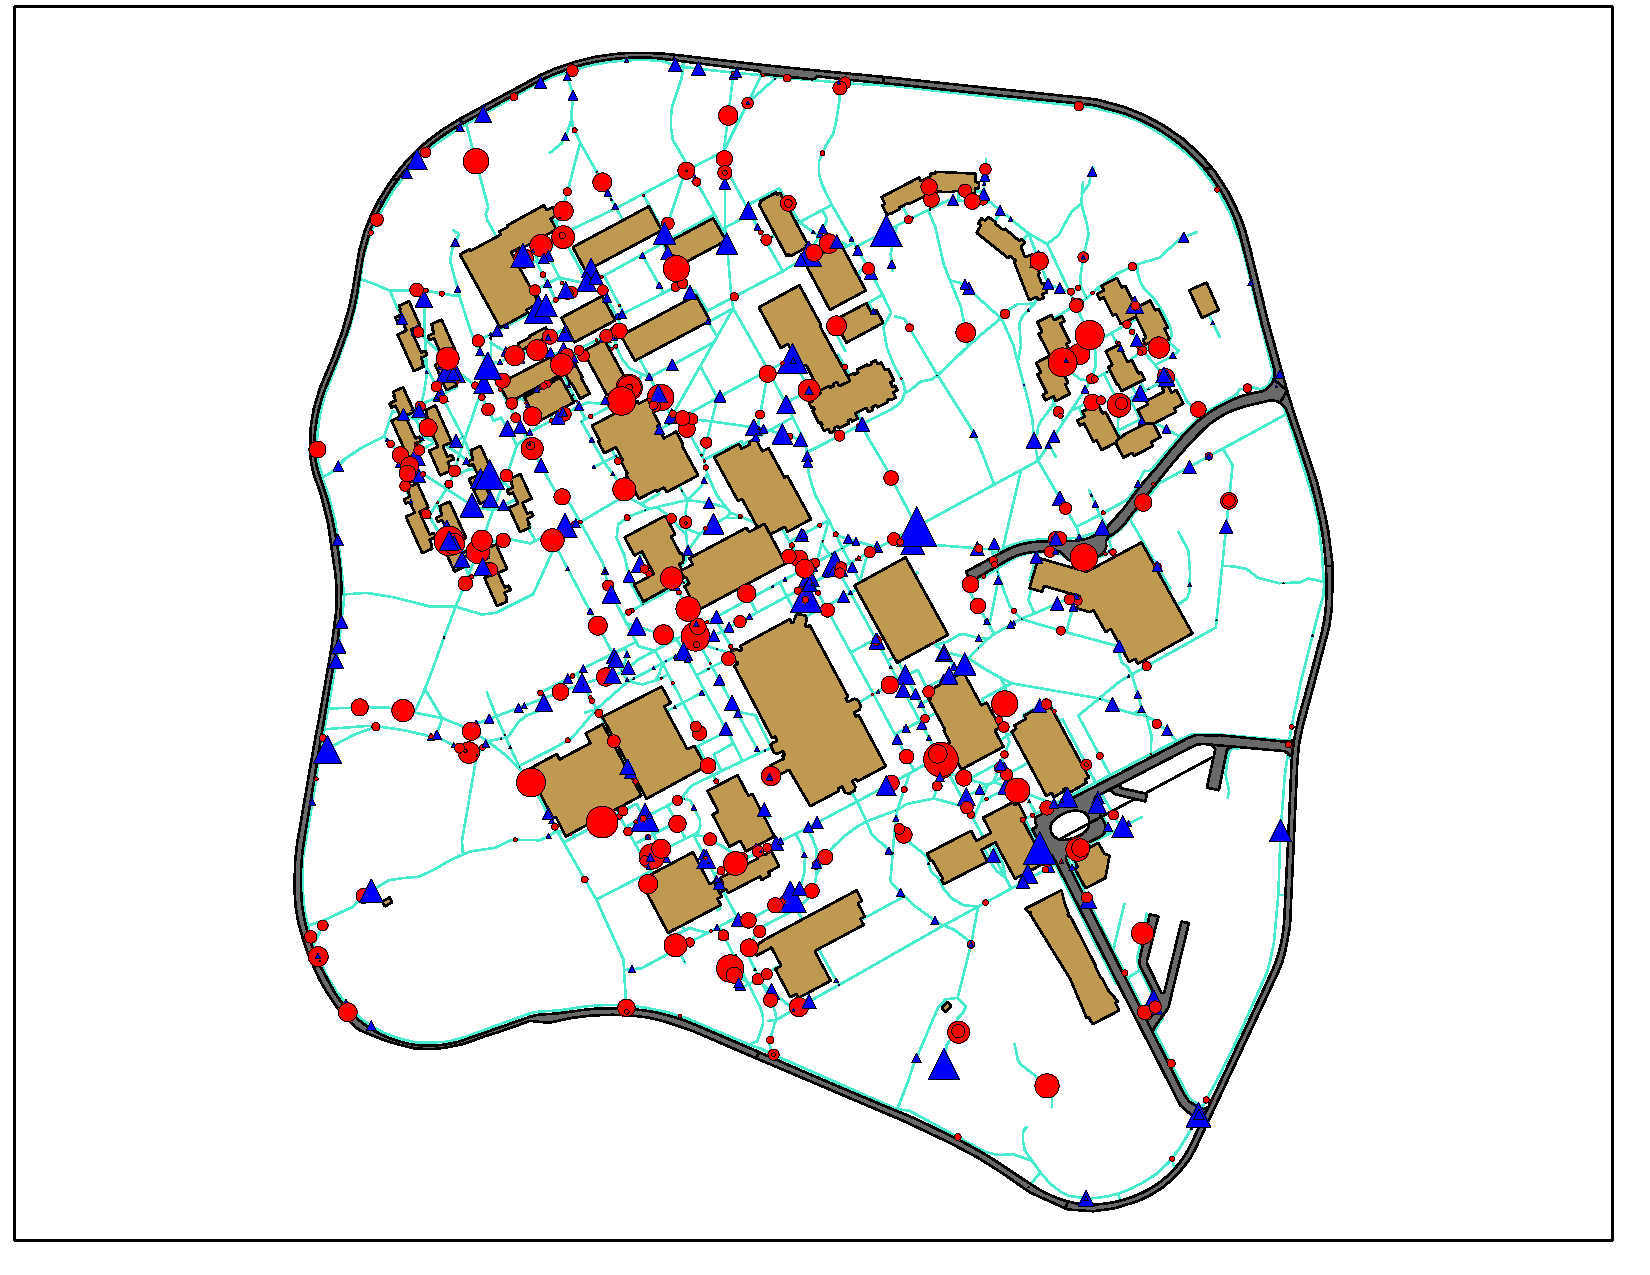
\includegraphics[width=0.75\textwidth]{CampusWorld.pdf}
  \caption{Snapshot of ``Campus World'' demo .}
  \label{fig:campusworld}
\end{figure}

Consider the GeoMason ``Campus World'' demo that has
agents moving along walkways.\footnote{This demo is included with
  GeoMason, and can be found as \file{sim.app.geo.campusworld}}  The buildings, walkways, and roads were
loaded from shape files, but the agents were created stochastically
from within the simulation and stored in their own \class{GeomVectorField}.  When the simulation ends a shape file
describing these agents is written out to a shape file that can be
loaded along with the original shape files for analysis.  These agents
have the following three attributes: their age, movement rate, and whether they are
student or faculty. Fig. \ref{fig:campusworld} depicts these shape files
after they were loaded into a GIS with the faculty agents rendered as blue triangles, students as
red dots, and their relative sizes scaled to their respective movement rates.

Shape files are not single files but are instead comprised of a few mandatory files with
the extensions \file{.shp}, \file{.dbf}, and \file{.idx}.  The first
argument to \method{ShapeFileExporter.write()} specifies the file name
prefix used to generate these files from the given
\class{GeomVectorField}.

There is an optional shape file that contains the coordinate reference
system and uses the file name extension \file{.prj}.  This function
does not write this file.\footnote{However, a future incarnation of
  GeoMason may do so.}  However, if the \class{GeomVectorField} was
itself sourced from a shape file, then its corresponding \file{.prj}
file can be copied over using the new file extension used in the call
to \method{write()}.  Alternatively, if the \class{GeomVectorField} was
\emph{not} read from a shape file, and so does not have a corresponding
\file{.prj} file, you may still be in luck if you loaded other vector
layers from shape files.  If that's the case, you can likely
arbitrarily use one of their \file{.prj} files.

If you want to automatically save a snapshot of a
\class{GeomVectorField} after each simulation run, you can place this
call to \method{write()} within \method{finish()} inside your
\class{SimState} subclass.
\end{description}



\subsection{Writing an ARC/Info ASCII Grid File}
\label{sub:writinggridfile}

\begin{description}
\item[Problem]~\\
You want to write GeoMason grid data to an ARC/Info ASCII Grid file.

\item[Solution]~\\
Create a \code{Writer} for the grid file and use \code{ArcInfoASCGridExporter.write()} to write the \code{GeomGridField}.
\begin{Verbatim}[frame=lines,framesep=5mm,commandchars=+\[\]]
try {
   BufferedWriter writer = new BufferedWriter( new FileWriter("foo.asc") );
   ArcInfoASCGridExporter.write(gridField, writer);
   writer.close();
} catch (IOException ex)  {
   /* handle exception */
}
\end{Verbatim}

\item[Discussion] ~\\
This recipe is useful for saving grid data from a simulation run such
that you can later import it into a GIS for analysis.

Unlike calls to \method{ArcInfoASCGridImporter.read()}, you do not
have to specify a data type.  Instead, the call to
\method{ArcInfoASCGridExporter.write()} automatically handles that
detail for you.

As in recipe \ref{sub:writingshapefile} you can place this snippet into
\method{finish()} to automatically write a grid file when the
simulation ends.
\end{description}




\chapter{Using Geospatial Data}
\label{ch:using}

In this chapter we discuss interacting with geospatial data using
GeoMason.  These kinds of interactions are mostly queries such as
asking in what political boundaries an agent is located or determining
nearby entities.

%\begin{figure}[h]\vspace{-33em}\hspace{30em}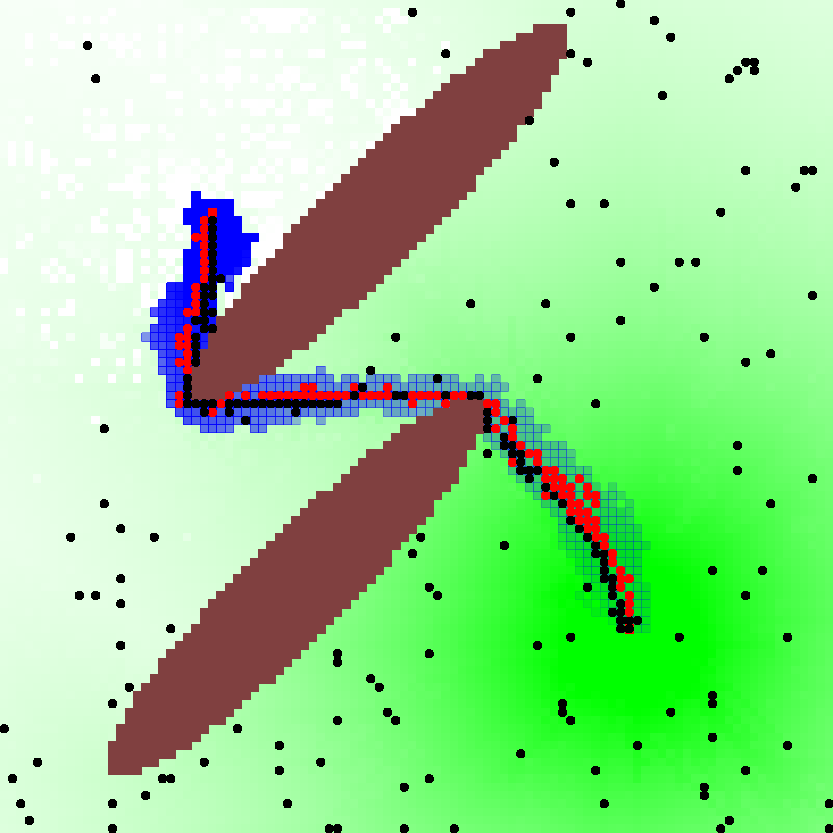
\includegraphics[width=4in]{ants.pdf}\vspace{2em}\end{figure}

\section{Determining What Political Entity an Agent is In}
\label{sec:politicalentity}

\begin{description}
\item[Problem]~\\
  You have a simulation with polygons for boundaries that delineate
  political entities such as countries, counties, or voting districts.
  In that simulation you also have agents that move across these kinds
  of boundaries, and you would like to know the political entity in
  which that agent is located.

\item[Solution]~\\
  Assume that a \class{GeomVectorField} contains the political
  boundary polygons.  If the agents are points in a
  \class{GeomVectorField}, then directly use their representative
  geometry to find what geometry covers them in the boundary vector
  field.  Alternatively, if the agents are in a \class{GeomGridField},
  then you can use the GeoMason grid field's \method{toPoint()} to
  convert from the grid coordinate to the underlying coordinate
  reference system, and then use that coordinate to find the boundary
  polygon that covers that point.

\begin{Verbatim}[frame=lines,label=Agents as Vector Field,framesep=5mm]
GeomVectorField boundaries = new GeomVectorField(WIDTH,HEIGHT);
GeomVectorField agents = new GeomVectorField(WIDTH,HEIGHT);

// ...

// Arbitrarily select first agent
MasonGeometry agent = (MasonGeometry) agents.getGeometries().objs[0];

// Bag should contain a single MasonGeometry object for polity in
// which agent is located.
Bag polity = boundaries.getCoveringObjects(agent.geometry);

if ( polity.isEmpty() ) {
   // the agent is not in any polity defined in boundaries
}
\end{Verbatim}

\begin{Verbatim}[frame=lines,label=Agents as Grid Field,framesep=5mm,commandchars=+\[\]]
GeomVectorField boundaries = new GeomVectorField(WIDTH,HEIGHT);
GeomGridField agents = new GeomGridField();

// ...

// (x,y) denotes an arbitrary valid location within the grid field, agents
+color[red]Point p = agents.toPoint(x, y);+label[ex:topoint]

// Again, Bag should contain a single MasonGeometry object for polity
// in which everything in that grid cell is located.
Bag polity = boundaries.getCoveringObjects(p);

if ( polity.isEmpty() ) {
   // the agent is not in any polity defined in boundaries
}
\end{Verbatim}

\item[Discussion ]~\\
Naturally all the various vector and grid layers should use the same
underlying coordinate reference system and should have their
respective \idx{minimum bounding rectangles} (MBR) synchronized as per
recipe \ref{sub:multiplevectorlayers}.

Note that the \code{isEmpty()} check may return true even if you think
that an agent should be in a given polity due to errors in the
underylying data.  E.g., the polygons between adjacent political
entities may not align perfectly leaving little ``void'' gaps in which
an agent can fall.  

% TODO this could benefit from ancillary graphic examples

Also, the center points of grids are used as reference points to
determine in which region a particular grid-based agent falls; some
grid cells that overlap polygon edges may have center points that fall
outside region polygons.  This sometimes means that the wrong
political region may be reported for a given grid cell.  If more
precision is required to avoid those scenarios, then instead of the
\method{toPoint()} call, which is highlighted above on line
\ref{ex:topoint}, you can use \method{toPolygon()} to return the
polygon outlining the corresponding grid cell.  You can then use that
polygon in the call to \method{getCoveringObjects()}.  However, be
aware that the returned \class{Bag} may contain multiple polygons
corresponding to regions that cover that grid cell's rectangular
coverage.  In which case you must then figure out which of the regions
the cell actually best covers.

\end{description}


\section{Locating Nearby Geospatial Objects}
\label{sec:nearbyobjects}

\begin{description}
\item[Problem]~\\
You want to find all the objects within a certain distance from a
specific thing.

\item[Solution]~\\
You can use \method{getObjectsWithinDistance()} to find all
objects within a certain distance from a given object.
\begin{Verbatim}[frame=lines,framesep=5mm,commandchars=+\[\]]
GeomVectorField objects = new GeomVectorField(WIDTH,HEIGHT);
Point location; // assume later set to desired location

// ...
	
Bag nearestObjects = objects.getObjectsWithinDistance(location,distance);

if (nearestObjects.isEmpty()) { System.out.println("Nothing nearby"); }
\end{Verbatim}

\item[Discussion]~\\
This recipe addresses finding geospatial objects in vector space.
Naturally if you want to locate nearby objects in a grid, you can use
the legacy MASON grid functions to locate nearby cells. \footnote{Do
  note that the MASON nearest neighbor functions are currently in
  flux, so use with caution.}
\end{description}


\section{Finding Adjacent Geospatial Objects}
\label{sec:findingadjacent}

\begin{description}
\item[Problem]~\\
You want to find adjacent geospatial objects. For example, for a given
country, you want to get a list of neighboring countries that share a
common border.

\item[Solution]~\\
This is very similar to recipe \ref{sec:nearbyobjects}.  Instead of
using \method{getObjectsWithinDistance()}  to find nearby objects, use
\method{getTouchingObjects()}, instead, to find bordering objects.
\begin{Verbatim}[frame=lines,framesep=5mm,commandchars=+\[\]]
GeomVectorField objects = new GeomVectorField(WIDTH,HEIGHT);
Point location; // assume later set to desired location

// ...
	
Bag nearestObjects = objects.getTouchingObjects(location);

if (nearestObjects.isEmpty()) { System.out.println("Nothing nearby"); }
\end{Verbatim}

\item[Discussion]~\\
  As for recipe \ref{sec:nearbyobjects}., this is for the vector
  domain.  Determining nearby objects in a grid is trivial to compute
  as they are just the adjacent grid cells.

  Again, as the description stated, this recipe can be used to compute
  adjacent polities.  Since those are generally static, you can
  compute the political entity adjacencies once when the simulation
  starts, and then store the values in a look-up table.
\end{description}


\section{Moving Agents Along Paths}
\label{sec:movingalongpaths}

\begin{description}
\item[Problem]~\\
You have a path, such as a road or trail, along which you want to move
an agent.

\item[Solution]~\\
  Presuming you are representing the paths as \class{LineString}s, you
  can create a corresponding \JTS
  \class{LengthIndexedLine} for each \class{LineString}.\footnote{If
    you have read in these line strings via a GeoMason importer, note
    that these \class{LineString}s will be wrapped in
    \class{MasonGeometry} objects stored in a
    \class{GeomVectorField}.} \class{LengthIndexedLine} allows you to
  ``index'' along its length; i.e., you can get a \JTSshort
  \class{Coordinate} for any position along a
  \class{LengthIndexedLine}.  So agents that are represented as points
  (i.e., coordinates), can get their current point position by
  indexing along a given \class{LengthIndexedLine}.  Each agent knows
  its index value for the current line it is on.  To move, the agent
  increments or decrements that index by some value corresponding to a
  movement rate --- the higher the value the faster the agent moves.
  It then gets the point for the position from its associated
  \class{LengthIndexedLine} and effects its movement by setting its
  point position to that value.

The following code is for a simple agent that moves back and forth along a single line segment.

\begin{Verbatim}[frame=lines,framesep=5mm,commandchars=^\[\]]
public class LineFollower implements Steppable
{
    // current position in 2D space
    private Coordinate position;

    // current index position along line
    private double currentIndex;

    // line along which agent is moving
    private LengthIndexedLine line;

    // how fast the agent moves along line
    private double moveRate = 1.0;

    public LineFollower(MasonGeometry geometry)
    {
        LineString lineString = (LineString) geometry.geometry;

        line = new LengthIndexedLine(lineString);

        // arbitrarily start at one end of the line
        currentIndex = line.getStartIndex();

        // update the 2D coordinate for that end of the line
        position = line.extractPoint(currentIndex);
    }

    @Override
    public void step(SimState state)
    {
        // If the next step takes us off the line, reverse course
        ^color[red]if (! line.isValidIndex(currentIndex + moveRate)) {^label[ex:validindex]
            moveRate *= -1;
        }

        currentIndex += moveRate;

        position = line.extractPoint(currentIndex);
    }
}
\end{Verbatim}

This example covers moving along a single line segment, which is
admittedly not very interesting. The next recipe,
\ref{sec:shortestpaths}, addresses navigating along line segment
networks.

\item[Discussion]~\\
  When incrementing or decrementing the \class{LengthIndexedLine}
  indices, ensure that you don't exceed the start or end point index
  values.  I.e., truncate them to the line start or end point value
  when a increment or decrement exceeds that value.  The highlighted
  line \ref{ex:validindex} demonstrates checking for stepping off the
  line segment.  If you want to move the agent on to a connecting line
  segment, then take the truncated balance and apply that to the index
  for the next \class{LengthIndexedLine}.

  \code{sim.app.geo.campusworld}, \code{sim.app.geo.gridlock}, and
  \code{sim.app.geo.networkworld} are GeoMason examples of agents
  moving along a line.
\end{description}


\section{Creating a Network Graph from Lines}
\label{sec:GraphFromLines}

\begin{description}
\item[Problem]~\\
You have a lines describing a network, such as roads, that you would like to have as a single network, or graph.

\item[Solution]~\\
GeoMason supplies a class, \class{GeomPlanarGraph}, that can be populated from a \class{GeomVectorField}.
\begin{Verbatim}[frame=lines,framesep=5mm,commandchars=+\[\]]
GeomVectorField vectorField = new GeomVectorField(WIDTH,HEIGHT);
// ...
GeomPlanarGraph graph = new GeomPlanarGraph();
graph.createFromGeomField(vectorField);
\end{Verbatim}

\item[Discussion]~\\
Once you have such a graph, it then becomes easier to compute shortest paths as in recipe \ref{sec:shortestpaths}.
\end{description}





\section{Calculating the Shortest Path on a Network}
\label{sec:shortestpaths}

\begin{description}
\item[Problem]~\\
You want to find the shortest path between two points in a network
such as set of roads.

\item[Solution]~\\
First, create a planar graph, as in recipe \ref{sec:GraphFromLines}.  Then use a shortest path algorithm, such as Dijkstra's\footnote{\url{http://en.wikipedia.org/wiki/Dijkstra\%27s_algorithm}} or $A^*$ \footnote{\url{http://en.wikipedia.org/wiki/A*_search_algorithm}} to compute the shortest route for each agent.

\item[Discussion]~\\
Computing shortest paths in a network is a well studied problem for which there exist a number of solutions, including solutions oriented towards transportation networks.\footnote{\url{http://en.wikipedia.org/wiki/Shortest_path_problem}}

Once the shortest path is computed you can use recipe \ref{sec:movingalongpaths} to move the agent along the route.

\item[See Also]~\\
The GridLock demo creates a GeomPlanarGraph and an $A^*$ algorithm to plot optimal commuter routes for agents.  This demo can be found at \file{sim.app.geo.gridlock}.
\end{description}


\section{Breaking Up Lines By Intersections}
\label{sec:NodingLines}

\begin{description}
\item[Problem]~\\
You want to ensure that lines are broken up by their intersections, which in \JTSshort parlance is otherwise known as ``noding''.

\item[Solution]~\\
  Create a \class{MultiLineString} from the set of lines of interest
  and then computing their \method{union()}.  The following is an
  example that uses this technique to split two lines that intersect
  in a 'T' formation into three line segments.

\begin{Verbatim}[frame=lines,framesep=5mm,numbers=left]
GeometryFactory geometryFactory = new GeometryFactory();
WKTReader reader = new WKTReader(geometryFactory);

ArrayList<LineString> rawlines = new ArrayList<LineString>();

rawlines.add((LineString) reader.read("LINESTRING (0 1, 1 1)"));
rawlines.add((LineString) reader.read("LINESTRING (1 0, 1 3)"));

MultiLineString newLines = 
    new MultiLineString(rawlines.toArray(new LineString[0]), geometryFactory);

System.out.println("Before computing intersection:\n" + newLines);

Geometry brokenUpLines = newLines.union();

System.out.println("Broken up by intersection:\n" + brokenUpLines);
\end{Verbatim}

The output from this code shows the two lines are now broken into three
lines split by the original two lines' intersection:

\begin{Verbatim}
Before computing intersections:
MULTILINESTRING ((0 1, 1 1), (1 0, 1 3))
Broken up by intersection:
MULTILINESTRING ((0 1, 1 1), (1 0, 1 1), (1 1, 1 3))
\end{Verbatim}

\JTSshort offers a third approach to computing line intersections.  You can
use a ``Noder'' that explicitly calculates the intersections between
all the given geometry as shown in the following example.

\begin{Verbatim}[frame=lines,framesep=5mm,numbers=left]
GeometryFactory geometryFactory = new GeometryFactory();
WKTReader reader = new WKTReader(geometryFactory);

MultiLineString multiLine = 
    (MultiLineString) reader.read("MULTILINESTRING ((0 1, 1 1),(1 3, 1 0))");

System.out.println("Before computing intersections: " + multiLine);

List lines = SegmentStringUtil.extractSegmentStrings(multiLine);

System.out.println("Converted to segmented lines: " + lines);

RobustLineIntersector RLI = new RobustLineIntersector();
IntersectionAdder SI = new IntersectionAdder(RLI);

MCIndexNoder noder = new MCIndexNoder();
noder.setSegmentIntersector(SI);

noder.computeNodes(lines);

System.out.println("Noded Noded Substrings: " + noder.getNodedSubstrings());
\end{Verbatim}

This code produces the following output:

\begin{Verbatim}
Before computing intersections: MULTILINESTRING ((0 1, 1 1), (1 3, 1 0))
Converted to segmented lines: [LINESTRING (0.0 1.0, 1.0 1.0), LINESTRING (1.0 3.0, 1.0 0.0)]
Noded Substrings: [LINESTRING (0.0 1.0, 1.0 1.0), LINESTRING (1.0 3.0, 1.0 1.0), 
   LINESTRING (1.0 1.0, 1.0 0.0)]}
\end{Verbatim}

Note that the noder returns a list of \class{NodedSegmentString}s,
which may be inconvenient.

\item[Discussion]~\\
  This is usually a prerequsite for computing line intersections,
  which is described in recipe \ref{sec:lineintersection}.  Though the
  examples are comprised entirely of \JTSshort objects, recall that
  you can access JTS \class{Geometry} objects via the
  \method{MasonGeometry.geometry} data member.
\end{description}


\section{Computing Line Intersections}
\label{sec:lineintersection}

\begin{description}
\item[Problem]~\\
  You want to find all the intersections for a set of lines.  For
  example, you may want to locate all road junctions.

\item[Solution]~\\
  Use the \JTS \class{Geometry} method
  \method{intersection()} to compute the intersecting
  \class{Point}. The following code gives an example of using
  \method{intersection()}.

\begin{Verbatim}[frame=lines,framesep=5mm,commandchars=^\[\]]
GeometryFactory geometryFactory = new GeometryFactory();
WKTReader reader = new WKTReader(geometryFactory);

LineString firstLine =
    (LineString) reader.read("LINESTRING (0 10, 10 10)");
LineString secondLine =
    (LineString) reader.read("LINESTRING (5 20, 5 0)");

^color[red]Geometry intersection = firstLine.intersection(secondLine);

System.out.println("Intersection of " + firstLine + " and " + secondLine + " is " + intersection);
\end{Verbatim}

The output of this code is ``Intersection of LINESTRING (0 10, 10 10)
and LINESTRING (5 20, 5 0) is POINT (5 10)'', as you would expect.

However, generally we're more interested in finding the intersections
for a set of lines.  Unfortnately we're not guaranteed that our data
is \emph{coplanar}; that is, that when lines cross one another that
they have an explicit vertex at that intersection. Before we can
compute the points for all the intersections, we must first ensure all
the data is coplanar.  Fortunately \JTSshort has ways of breaking up lines
by their intersections.  This can be done by 
Once we're guaranteed that the lines are coplanar, we then need to
find the points that define the line network intersections.  You can
do this getting the line start and end point coordinates, and then
noting which of those occur more than once; those would be the
points corresponding to line intersections.

The following code takes lines noded from the previous code example
that uses the \class{MCIndexNoder} and prints the intersection value.

\begin{Verbatim}[frame=lines,framesep=5mm,numbers=left]
// contains noded line strings
Collection nodedLines = noder.getNodedSubstrings();

Set<Coordinate> intersectionVertices = new HashSet<Coordinate>();
Set<Coordinate> visitedCoordinates = new HashSet<Coordinate>();

for (Object line : nodedLines.toArray()) {
    NodedSegmentString curLine = (NodedSegmentString) line;

    Coordinate [] coordinates = curLine.getCoordinates();

    // Start point
    if (! visitedCoordinates.contains(coordinates[0])) {
        visitedCoordinates.add(coordinates[0]);
    } else {
        intersectionVertices.add(coordinates[0]);
    }

    // End point
    if (! visitedCoordinates.contains(coordinates[coordinates.length - 1])) {
        visitedCoordinates.add(coordinates[coordinates.length - 1]);
    } else {
        intersectionVertices.add(coordinates[coordinates.length - 1]);
    }
}

for (Coordinate c : intersectionVertices.toArray(new Coordinate[0])) {
    System.out.println(c);
}
\end{Verbatim}

The output is (1.0, 1.0, NaN), which is what we'd expect.  (The NaN is
for the Z coordinate, which isn't used in GeoMason.)

\JTSshort does provide a simple one off means of getting line segment
intersections.  The following code demonstrates this;
\code{brokenUpLines} is the noded \JTSshort \class{MultiLineString}
from the example that used \method{union()}.\footnote{Thanks to Martin
  Davis, the JTS author, for this example.}

\begin{Verbatim}[frame=lines,framesep=5mm,numbers=left]
System.out.println("Noded Substrings: " + brokenUpLines);

Geometry intPoints = (new BoundaryOp(brokenUpLines, 
    BoundaryNodeRule.MULTIVALENT_ENDPOINT_BOUNDARY_RULE)).getBoundary();

System.out.println("Intersection: " + intPoints);
\end{Verbatim}

The output from this is: 
\begin{Verbatim}
Noded Substrings: MULTILINESTRING ((0 1, 1 1), (1 3, 1 1), (1 1, 1 0))
Intersection: POINT (1 1)
\end{Verbatim}

\item[Discussion]~\\
% GeoMason uses the \JTS to represent the
%   underlying geometry and to provide geometry operations.  One such
%   operation is for computing intersections.  To that end, each
%   \JTSshort \class{Geometry} has a method, \method{intersection()},
%   that returns a \class{Geometry} object that corresponds to the
%   intersection between the two given geometries; in the case of a
%   \class{LineString} the returned intersecting object is a
%   \class{Point}.  The returned \class{Geometry} will be empty, which
%   is checked by calling \method{isEmpty()}, if the two geometries do
%   not intersect.  
  Note that the \JTSshort \class{Geometry} can be directly accessed from
  wrapping \class{MasonGeometry} objects as the \member{geometry}
  member.
\end{description}




\section{Calculating Agent Information from Underlying Grid Data}
\label{sec:gridtoagentdata}

\begin{description}
\item[Problem]~\\
You wish to to compute something based on values found in a grid an
agent occupies.  For example, a grid may represent a hectare and an
agent may want to consume certain amount of vegetation and water found there.

\item[Solution]~\\
Assume that you have an agent in a \class{GeomVectorField} and a
corresponding \class{GeomGridField} layer that has information that
agent needs to get or modify.  First, you need to determine the
grid cell coordinate for the agent.  Then you can use that coordinate
to fetch the grid cell contents.
\begin{Verbatim}[frame=lines,framesep=5mm,numbers=left]
GeomVectorField agent = new GeomVectorField(WIDTH,HEIGHT);
GeomGridField gridField = new GeomGridField();

// ... assume agent and gridField populated at this point

// assume first object in agent layer corresponds to agent of interest
Point location = agent.getGeometries().objs[0];

int x = gridField.toX(location);
int y = gridField.toY(location);

// assume grid field is of integers
int value = ((IntGrid2D)gridField.getGrid()).get(x,y);
\end{Verbatim}

\item[Discussion]~\\
Naturally the above code example can be generalized to cover the other
MASON 2D grid types.

This assumes that the grid and vector layers have the same underlying
coordinate reference system and have had their minimum bounding
rectangles synchronized as per recipe \ref{sub:readingmixofdata}.

In a way, this is the inverse of recipe \ref{sec:politicalentity} ---
that is, instead of going from a grid layer to a vector, we're going
from a vector to the grid.
\end{description}



\section{Having an Agent Follow a Gradient}
\label{sec:followinggradients}

\begin{description}
\item[Problem]~\\
You have slope information that you would like an agent to follow.

\item[Solution]~\\
  Let's assume that you have a grid file containing elevation postings;
  i.e., essentially a matrix of floating point values that denote a
  height.  An agent can be an arbitrary point associated with the
  elevation grid that's initialized at some random location.  For each
  time step, the agent can get the height from its corresponding grid
  cell, and then find the adjacent cell with the smallest height and
  then move to that cell.  The code below is a simple implementation
  of this approach.

\begin{Verbatim}[frame=lines,framesep=5mm,commandchars=^\[\]]
public class Gradient extends SimState
{
    // field of elevation data
    GeomGridField elevation = new GeomGridField();

    // denotes agent's location; randomly set in start()
    int agentX;
    int agentY;

    public Gradient(long seed)
    {
        super(seed);

        InputStream elevationInputStream = null;

        try
        {
            elevationInputStream = new FileInputStream("elevations.asc");
        } catch (FileNotFoundException ex)
        {
            Logger.getLogger(Gradient.class.getName()).log(Level.SEVERE, null, ex);
        }

        ArcInfoASCGridImporter.read(elevationInputStream, GridDataType.DOUBLE, elevation);
    }


    @Override
    public void start()
    {
        super.start();

        // randomly place agent
        agentX = random.nextInt(elevation.getGridWidth());
        agentY = random.nextInt(elevation.getGridHeight());

        schedule.scheduleRepeating(new Mover());
    }


    // Steppable that moves the agent down slope
    private class Mover implements Steppable
    {
        public Mover()
        {}

        // heights of nearby cells
        DoubleBag heights = new DoubleBag();^label[ex:doublebag]

        // Xs of nearby cells
        IntBag Xs = new IntBag();^label[ex:intbag1]

        // Ys of nearby cells
        IntBag Ys = new IntBag();^label[ex:intbag2]


        @Override
        public void step(SimState state)
        {
            Gradient gradient = (Gradient) state;

            // first get the adjacent eight cells and current cell

            heights = ((DoubleGrid2D)
            elevation.getGrid()).getNeighborsHamiltonianDistance(gradient.agentX,
                                                                 gradient.agentY,
                                                                 1, // distance
                                                                 false, // not torodial
                                                                 heights, Xs, Ys);

            // now find the cell with the lowest height

            int indexOfMin = 0; // index of heights with lowest elevation

            double currentMin = heights.get(0); // current lowest elevation

            for (int i = 1; i < heights.size(); i++) {
                if (heights.get(i) < currentMin) { 
                  indexOfMin = i;
                  currentMin = heights.get(i);
                }
            }

            // Now set agent coordinate to minimum
            gradient.agentX = Xs.get(indexOfMin);
            gradient.agentY = Ys.get(indexOfMin);
        }
    }
}
\end{Verbatim}

Note that as an optimization the \class{DoubleBag} and \class{IntBag}
objects in \code{Mover} in lines \ref{ex:doublebag}, \ref{ex:intbag1},
and \ref{ex:intbag2} are declared outside of \method{step()} so that
they are re-used instead of being recreated with each simulation step.

\item[Discussion]~\\
  The Water World demo, found as \code{sim.app.geo.waterworld}, gives
  a more elaborate example of how to follow a gradient.  This demo
  uses elevation data for Crater Lake, Oregon, in a water flow model.
  In this model, rain drops are randomly dropped onto the grid; some
  of the rain drops fill the cadera while the rest runs down the
  gradients. Additionally, once the water level exceeds the height of
  the rim, the crater water then flows down streams from the crater.

  The silly peds model is another gradient descent-based model.  It
  overlays a building floor plan onto a grid of heights; the agents
  follow the height gradient out of the building.  This demo can be
  found as \code{sim.app.geo.sillypeds}.

  Fig. \ref{fig:gradients} shows screenshots of both of these demos.
\end{description}

\begin{figure}[th]
  \centering
  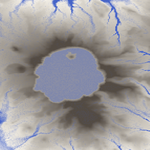
\includegraphics[width=0.45\textwidth]{WaterWorld.png}
  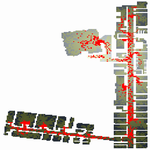
\includegraphics[width=0.45\textwidth]{SillyPeds.png}
  \caption{Screenshots of WaterWorld and SillyPeds models.}
  \label{fig:gradients}
\end{figure}






%%
%%
%%

\chapter{Displaying Geospatial Data}
\label{ch:displaying}

This chapter gives recipes for displaying GeoMason fields in MASON.

%\begin{figure}[h]\vspace{-26em}\hspace{25.3em}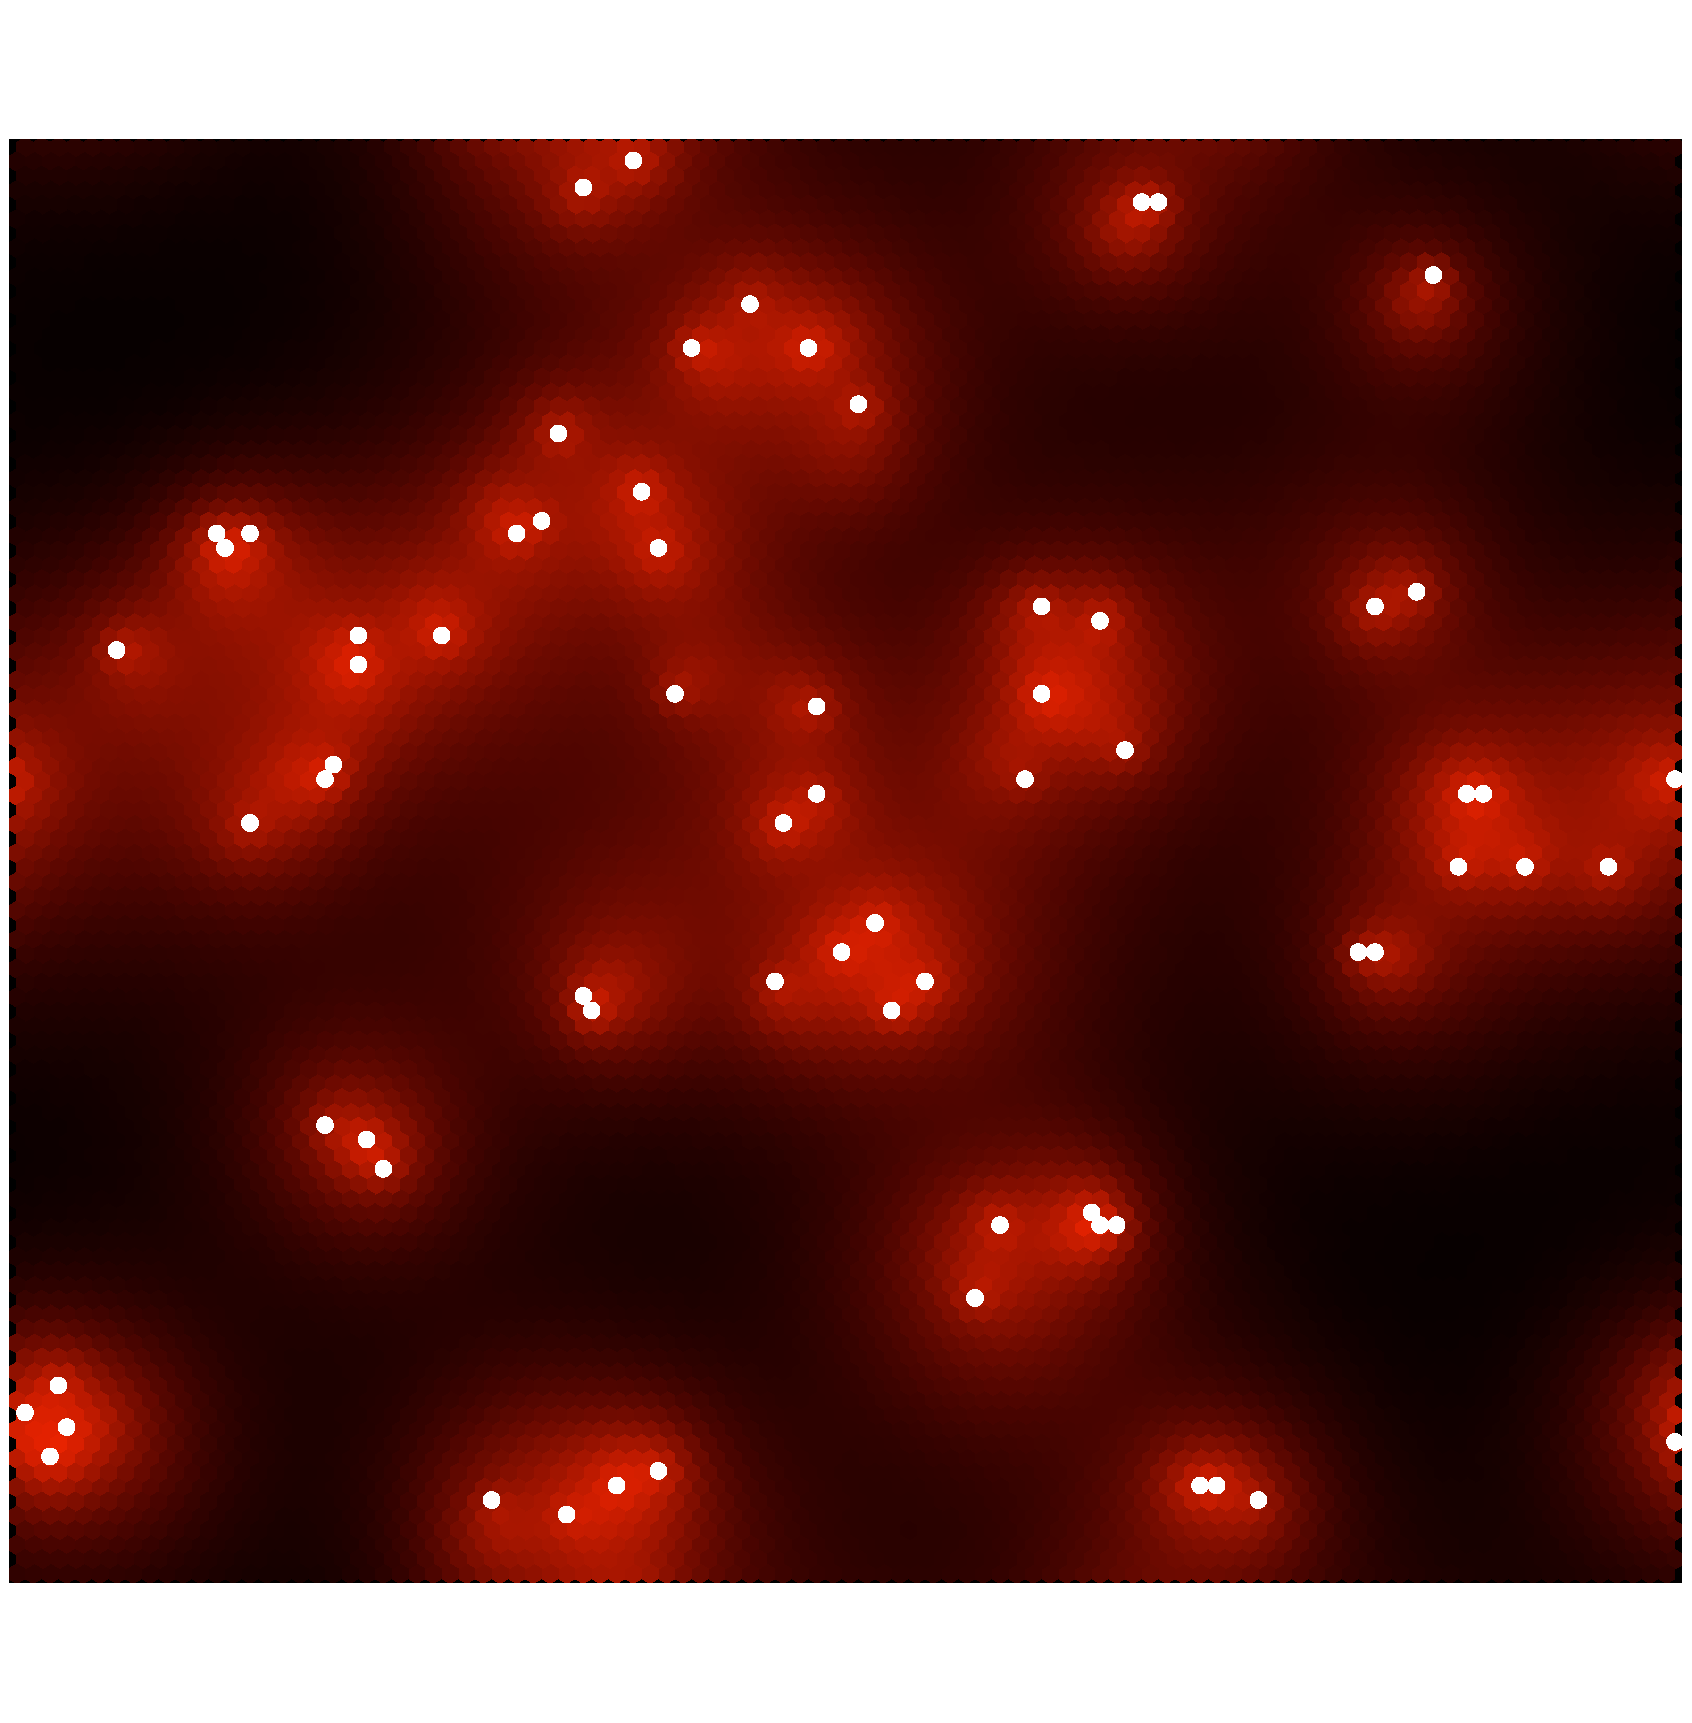
\includegraphics[width=4in]{hexabugs.pdf}\vspace{2em}\end{figure}

%\noindent A {\bf grid} is MASON's name for objects arrange in a 2-dimensional or 3-dimensional array or equivalent.  MASON supports a wide range of grid environments as fields (representations of space).  This includes most any combination of the following:

\section{Displaying a \code{GeomVectorField}}
\label{sec:displayingGeomVectorField}

\begin{description}
\item[Problem]~\\
You want to show the contents of a \code{GeomVectorField} in a
MASON display.

\item[Solution]~\\
Create a \code{GeomVectorFieldPortrayal} in the MASON \code{GUIState}
subclass, associate it with its corresponding \code{GeomVectorField},
set up an appropriate MASON or GeoMason field portrayal, and attach it
to a MASON \code{Display2D} object.

\begin{Verbatim}[frame=lines,framesep=5mm,commandchars=+\[\]]
public class MyMasonGUI extends GUIState
{
    private Display2D display;
    private JFrame displayFrame;

    // ... other variable declarations

    +color[red]private GeomVectorFieldPortrayal myPortrayal = new GeomVectorFieldPortrayal();

    @Override
    public void init(Controller controller)
    {
        super.init(controller);

        display = new Display2D(ARBITRARY_WIDTH, ARBITRARY_HEIGHT, this);

        +color[red]display.attach(myPortrayal, "My Vector Layer");

        displayFrame = display.createFrame();
        controller.registerFrame(displayFrame);
        displayFrame.setVisible(true);
    }

    @Override
    public void start()
    {
        super.start();
        setupPortrayals();
    }

    private void setupPortrayals()
    {
        MyState world = (MyState)state;

        +color[red]myPortrayal.setField(world.vectorLayer);
        +color[red]myPortrayal.setPortrayalForAll(new GeomPortrayal(Color.CYAN, true));+label[ex:trueforfill]

        display.reset();
        display.setBackdrop(Color.WHITE);

        display.repaint();
    }

    // ... other code
}
\end{Verbatim}

\item[Discussion ]~\\

Line \ref{ex:trueforfill} creates a portrayal that draws all the lines
in cyan; the optional second parameter, which is set to \code{true}, indicates
that polygons should be filled.  

Another optional parameter, which is not shown in the above example,
is for the scale to which geometry should be drawn.  Care should be
given when setting this parameter as the scale is in the units of the
underling coordinate reference system. For example, this means that if
you are using UTM all geometry will be in scaled to a be in meters, or
in degrees if you are using lat/lon coordinates.  If you are not
careful, you can have scale values that either render geometry so
small so as to not be visible, or so large as to obscure the entire
display. Note that by default the scale value is 1, which may be too
small if the simulation area is quite large and the units are in
meters; conversely it may be too large if the units are in degrees.
Some experimentation for the correct scale value may be
necessary. Recipe \ref{sec:OneColorDisplay} addresses problems
associated with bad \class{GeomPortrayal} scale factor values.

Note that legacy MASON potrayals can be used.  E.g., if you have
agents represented as points in a \class{GeomVectorField} you might
decide to use a MASON \class{RectanglePortrayal2D} instead of \class{GeomPortrayal}.

% Also, make a
% note of the scale factor given the units of the coordinate reference system.
\end{description}





\section{Displaying a \code{GeomGridField}}
\label{sec:displayinggridfield}

\begin{description}
\item[Problem]~\\
You want to show the contents of a \code{GeomGridField} in a MASON display

% TODO Add in MyState to exemplify
\item[Solution]~\\
Set up an appropriate field portrayal for the wrapped \class{Grid2D}
object found inside the \class{GeomGridField} .
\begin{Verbatim}[frame=lines,framesep=5mm,commandchars=+\[\]]
public class MyMasonGUI extends GUIState
{
    private Display2D display;
    private JFrame displayFrame;

    // ... other variable declarations

    +color[red]private FastValueGridPortrayal2D myPortrayal = new FastValueGridPortrayal2D();+label[ex:gridportrayal]

    @Override
    public void init(Controller controller)
    {
        super.init(controller);

        display = new Display2D(ARBITRARY_WIDTH, ARBITRARY_HEIGHT, this);

        +color[red]display.attach(myPortrayal, "My Grid Layer");

        displayFrame = display.createFrame();
        controller.registerFrame(displayFrame);
        displayFrame.setVisible(true);
    }

    @Override
    public void start()
    {
        super.start();
        setupPortrayals();
    }

    private void setupPortrayals()
    {
        MyState world = (MyState)state;

        +color[red]myPortrayal.setField(world.gridLayer.getGrid());+label[ex:getgrid]
        +color[red]myPortrayal.setMap(new SimpleColorMap(0, 1, Color.black, Color.white)); +label[ex:gridcolormap]

        display.reset();
        display.setBackdrop(Color.WHITE);

        display.repaint();
    }

    // ... other code
}

\end{Verbatim}

\item[Discussion ]~\\
% TODO add reference to MASON manual and emphasize that usual MASON 
A \class{GeomGridField} is effectively a wrapper round a MASON
\class{Grid2D} object, which means you can use the display techniques
for \class{Grid2D} objects.  Just use the
\method{GeomGridField.getGrid()} method to fetch the underlying
\class{IntGrid2D} or \class{DoubleGrid2D} object, as appropriate for
the data type you specified when you read the grid data.  (See recipe
\ref{sub:readinggridfile} for how to specify the grid data
representation.)

The above code sample is for reading a grid layer that's presumably
comprised of just ones and zeroes.  So a
\class{FastValueGridPortrayal2D} will suffice to render that layer, as
shown in line \ref{ex:gridportrayal}, along with an associated \class{SimpleColorMap} to show the zeros in
black and the ones in white, as seen in line \ref{ex:gridcolormap}.
The grid is attached to the field as in non-GeoMason MASON simulations;
line \ref{ex:getgrid} shows the \method{getGrid()} call necessary to get at the underyling
MASON \class{IntGrid2D}.
\end{description}



\section{Displaying Boundary Lines Over a Grid Field}
\label{sec:boundaryovergrid}

\begin{description}
\item[Problem]~\\
You want to overlay political boundaries on grid data.

\item[Solution]~\\
Load the vector and grid layers as per recipe
\ref{sub:readingmixofdata}.  Then set up the portrayals such that the
vector layer is rendered on top of the raster layer.

\begin{Verbatim}[frame=lines,label=Reading the layers,framesep=5mm,commandchars=+\[\]]
GeomVectorField boundaries = new GeomVectorField(WIDTH,HEIGHT);
GeomGridField gridField = new GeomGridField();

try {
   ShapeFileImporter.read("file:boundaries.shp", boundaries);

   InputStream inputStream = new FileInputStream("grid.asc");
   ArcInfoASCGridImporter.read(inputStream, GridDataType.INTEGER, gridField);
} catch (FileNotFoundException ex)
{  /* handle exception */  }

Envelope globalMBR = boundaries.getMBR();

globalMBR.expandToInclude(gridField.getMBR());

boundaries.setMBR(globalMBR);
gridField.setMBR(globalMBR);
\end{Verbatim}

\begin{Verbatim}[frame=lines,label=Displaying boundaries over the grid,framesep=5mm,commandchars=+\[\]]
public class MyMasonGUI extends GUIState
{
    private Display2D display;
    private JFrame displayFrame;

    // ... other variable declarations

    private FastValueGridPortrayal2D gridPortrayal = new FastValueGridPortrayal2D();
    private GeomVectorFieldPortrayal boundariesPortrayal = new GeomVectorFieldPortrayal();

    @Override
    public void init(Controller controller)
    {
        super.init(controller);

        display = new Display2D(ARBITRARY_WIDTH, ARBITRARY_HEIGHT, this);

        display.attach(gridPortrayal, "My Grid Layer");
        display.attach(boundariesPortrayal, "Political Boundaries");

        displayFrame = display.createFrame();
        controller.registerFrame(displayFrame);
        displayFrame.setVisible(true);
    }

    @Override
    public void start()
    {
        super.start();
        setupPortrayals();
    }

    private void setupPortrayals()
    {
        MyState world = (MyState)state;

        myPortrayal.setField(world.gridField.getGrid());
        myPortrayal.setMap(new SimpleColorMap(0, 1, Color.black, Color.white));

        myPortrayal.setField(world.boundaries);
        myPortrayal.setPortrayalForAll(new GeomPortrayal(Color.GRAY, true));

        display.reset();
        display.setBackdrop(Color.WHITE);

        display.repaint();
    }

    // ... other code
}
\end{Verbatim}

\item[Discussion]~\\
From the perspective of the \class{GUIState}, the vector layer of boundaries are just
yet another field portrayal rendered on top of another showing grid
data.  If the minimum bounding rectangles (MBR) of the two fields were
properly aligned --- and that they have the same coordinate reference
system! --- then the boundaries should match up with the grid
layer geospatial features.

You can load additional grid layers before the vector layer, and you can
toggle their visibility in the MASON \class{Display2D} window.  It's
similarly possible to load multiple boundaries, though admittedly
displaying them all at once may be confusing; however, this confusion
may be somewhat mitigated with good choices for line colors and
widths.  Just ensure that the vector layers always are
\method{attach()}'d \emph{after} all the grid layers because otherwise
the grid layers will obscure the boundaries.
\end{description}



\section{Displaying a Dynamic Choropleth Map}
\label{sec:chroplethmap}

\begin{description}
\item[Problem]~\\
You want to create a dynamic choropleth map with colors changing based
on agent behavior.

\item[Solution]~\\
Have one \class{GeomVectorField} for agents and another containing
political boundary polygons. Create a \class{MasonGeometry} subclass
to be used for the political boundary polygons that will count the
agents that are within its borders.  Create a corresponding
\class{GeomPortrayal} subclass that scales the color according to the
agent count reported by that \class{MasonGeometry} subclass.

The following code shows how to use the special \class{MasonGeometry} subclass
when reading the shape file.  The highlighted lines shows that the
\code{class} object for the counting wrapper \class{MasonGeometry} is
passed in to \method{read()} so that that class is used instead of the
default \class{MasonGeometry}.

\begin{Verbatim}[frame=lines,label=In Your \class{SimState},framesep=5mm,commandchars=+\[\]]
public class MyWorld extends SimState {

    // used in GUIState to set up ColorMap
    public static int NUM_AGENTS = 20;

    public GeomVectorField borders = new GeomVectorField(WIDTH,HEIGHT);

    // public static so CountingMasonGeometry can access
    public static GeomVectorField agents = new GeomVectorField(WIDTH,HEIGHT);

    public MyWorld(long seed) {
        super(seed);

        URL politicalBoundaries = MyWorld.class.getResource("borders.shp");

        try {
            +color[red]ShapeFileImporter.read(politicalBoundaries, border, CountingGeomWrapper.class);
        } catch (FileNotFoundException ex) {
            // handle exception
        }
    }

    // ... other code
}
\end{Verbatim}

This is the class that is a wrapper round \class{MasonGeometry}.  It
just counts the number of agents that the given geometry ``covers'';
i.e., the agents that are within the boundaries of this object.

\begin{Verbatim}[frame=lines,label=\class{MasonGeometry} subclass that
  counts agents,framesep=5mm,commandchars=+\[\]]
public class CountingGeomWrapper extends MasonGeometry {
    public CountingGeomWrapper()  {
        super();
    }

    public int numAgentsInGeometry()  {
        Bag coveredAgents = MyWorld.agents.getCoveredObjects(this);
        return coveredAgents.numObjs;
    }
}
\end{Verbatim}

This portrayal doesn't do anything special.  It just takes the number
of agents from the special counting \code{MasonGeometry} object to
lookup the appropriate color in the color map, and then renders the
overall geometry using that color.

\begin{Verbatim}[frame=lines,label=Portrayal that renders choropleth,framesep=5mm,commandchars=+\[\]]
public class WorldPortrayal extends GeomPortrayal {

    SimpleColorMap colorMap = null; 
	
    public WorldPortrayal(SimpleColorMap map) {
        super(true); 
        colorMap = map; 
    }
	
    @Override
    public void draw(Object object, Graphics2D graphics, DrawInfo2D info) {
       +color[red]CountingGeomWrapper gm = (CountingGeomWrapper)object;
       +color[red]paint = colorMap.getColor(gm.numAgentsInGeometry());
       super.draw(object, graphics, info);    
    }
}
\end{Verbatim}

And, finally, in the \class{GUIState} class, the appropriate
\class{GeomVectorFieldPortrayal} is set up to use our special field
portrayal with a color map based on the total number of agents in the simulation.

\begin{Verbatim}[frame=lines,label=Set up portrayal in \class{GUIState},framesep=5mm,commandchars=+\[\]]
    GeomVectorFieldPortrayal borderPortrayal = new GeomVectorFieldPortrayal();
    GeomVectorFieldPortrayal agentPortrayal = new GeomVectorFieldPortrayal();

    private void setupPortrayals()   {
        MyWorld world = (MyWorld) state;

        agentPortrayal.setField(MyWorld.agents);
        agentPortrayal.setPortrayalForAll(new OvalPortrayal2D(Color.RED, 6.0));

       +color[red] countyPortrayal.setField(world.borders);
       +color[red] countyPortrayal.setPortrayalForAll(new MyWorldPortrayal(
            +color[red]new SimpleColorMap(0.0, MyWorld.NUM_AGENTS, Color.WHITE, Color.BLUE)));

        display.reset();
        display.setBackdrop(Color.WHITE);
        display.repaint();
    }
\end{Verbatim}


\item[Discussion]~\\
Fig. \ref{fig:colorworld} shows a snapshot of the ``ColorWorld'' demo
the shows a choropleth of the Fairfax County voting districts; the
blue shading is in proportion to the number of agents that happen to
be within a given voting district at each time step.  This demo can be
found as \file{sim.app.geo.colorworld}.

Again, this above code exemplifies the approach that the ``ColorWorld'' demo uses ---
almost certainly there are other equally viable approaches to
implementing dynamic choropleths in GeoMason.

\begin{figure}[ht]
  \centering
  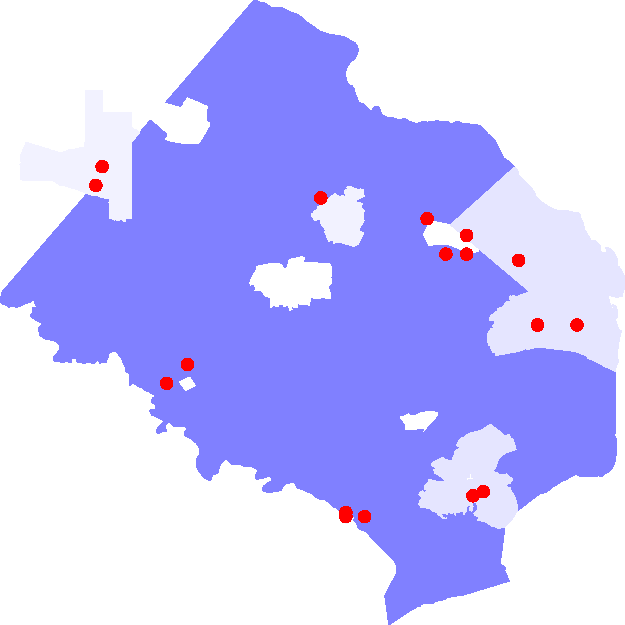
\includegraphics[width=0.75\textwidth]{ColorWorld.pdf}
  \caption{Snapshot of ``Color World'' demo showing polygon shading in
    proportion to number of agents.}
  \label{fig:colorworld}
\end{figure}

\end{description}


% XXX This recipe could perhaps be fleshed out a little more

\section{Displaying Raster Overlays}
\label{sec:displayingrasteroverlays}

\begin{description}
\item[Problem]~\\
  You have raster overlays you wish to render on top of other display
  layers.  For example, you may wish to overlay a heatmap representing
  population size, however you don't want the heatmap to hide details
  beneath it.

\item[Solution]~\\
You can use alpha transparency when creating the grid field portrayal.  

\begin{Verbatim}[frame=lines,framesep=5mm,numbers=left]
// Map population of grid cell from [0,25000] to shades of red from [0,255] with 
// alpha transparency of 100/255.
myPortrayal.setMap(new SimpleColorMap(0, 25000, new Color(0,0,0,100), new Color(255,0,0,100)));
\end{Verbatim}

\item[Discussion]~\\
Some experimentation may be necessary to determine the optimal alpha transparency level.
\end{description}






%%
%%
%%

\chapter{Common Problems}
\label{ch:commonprobs}


\section{Display All One Color}
\label{sec:OneColorDisplay}

\begin{description}
\item[Problem]~\\
Rendering a \code{GeomField} just shows one solid color.

\item[Solution]~\\
It is likely that the scale factor you are using for your
\class{GeomPortrayal} is too large.  Try using a scale factor that
makes sense for the underlying coordinate reference system.  E.g., if
you are using UTM, the units will be in meters; calculate the total
display area in meters and scale the agents accordingly.

See also recipe \ref{sec:displayingGeomVectorField}.
% \begin{Verbatim}[frame=lines,framesep=5mm,commandchars=+\[\]]
% foo
% \end{Verbatim}

\item[Discussion]~\\
Fig. \ref{fig:properscalefactor} shows the GeoMason Grid Lock demo. The left
subfigure shows the demo with the scale factor properly tailored to
the scale of the underlying coordinate reference system.  The right
subfigure shows what happens if you go with the default scale factor
of 1.0: the agents now obscure most of the display.  You can hopefully
see pathological variants where the agents cover the entire display in
a single color.  In this case we at least have a clue with part of the
Virginia road network peeping out from behind the rendered agents.
\begin{figure}[ht]
  \centering
  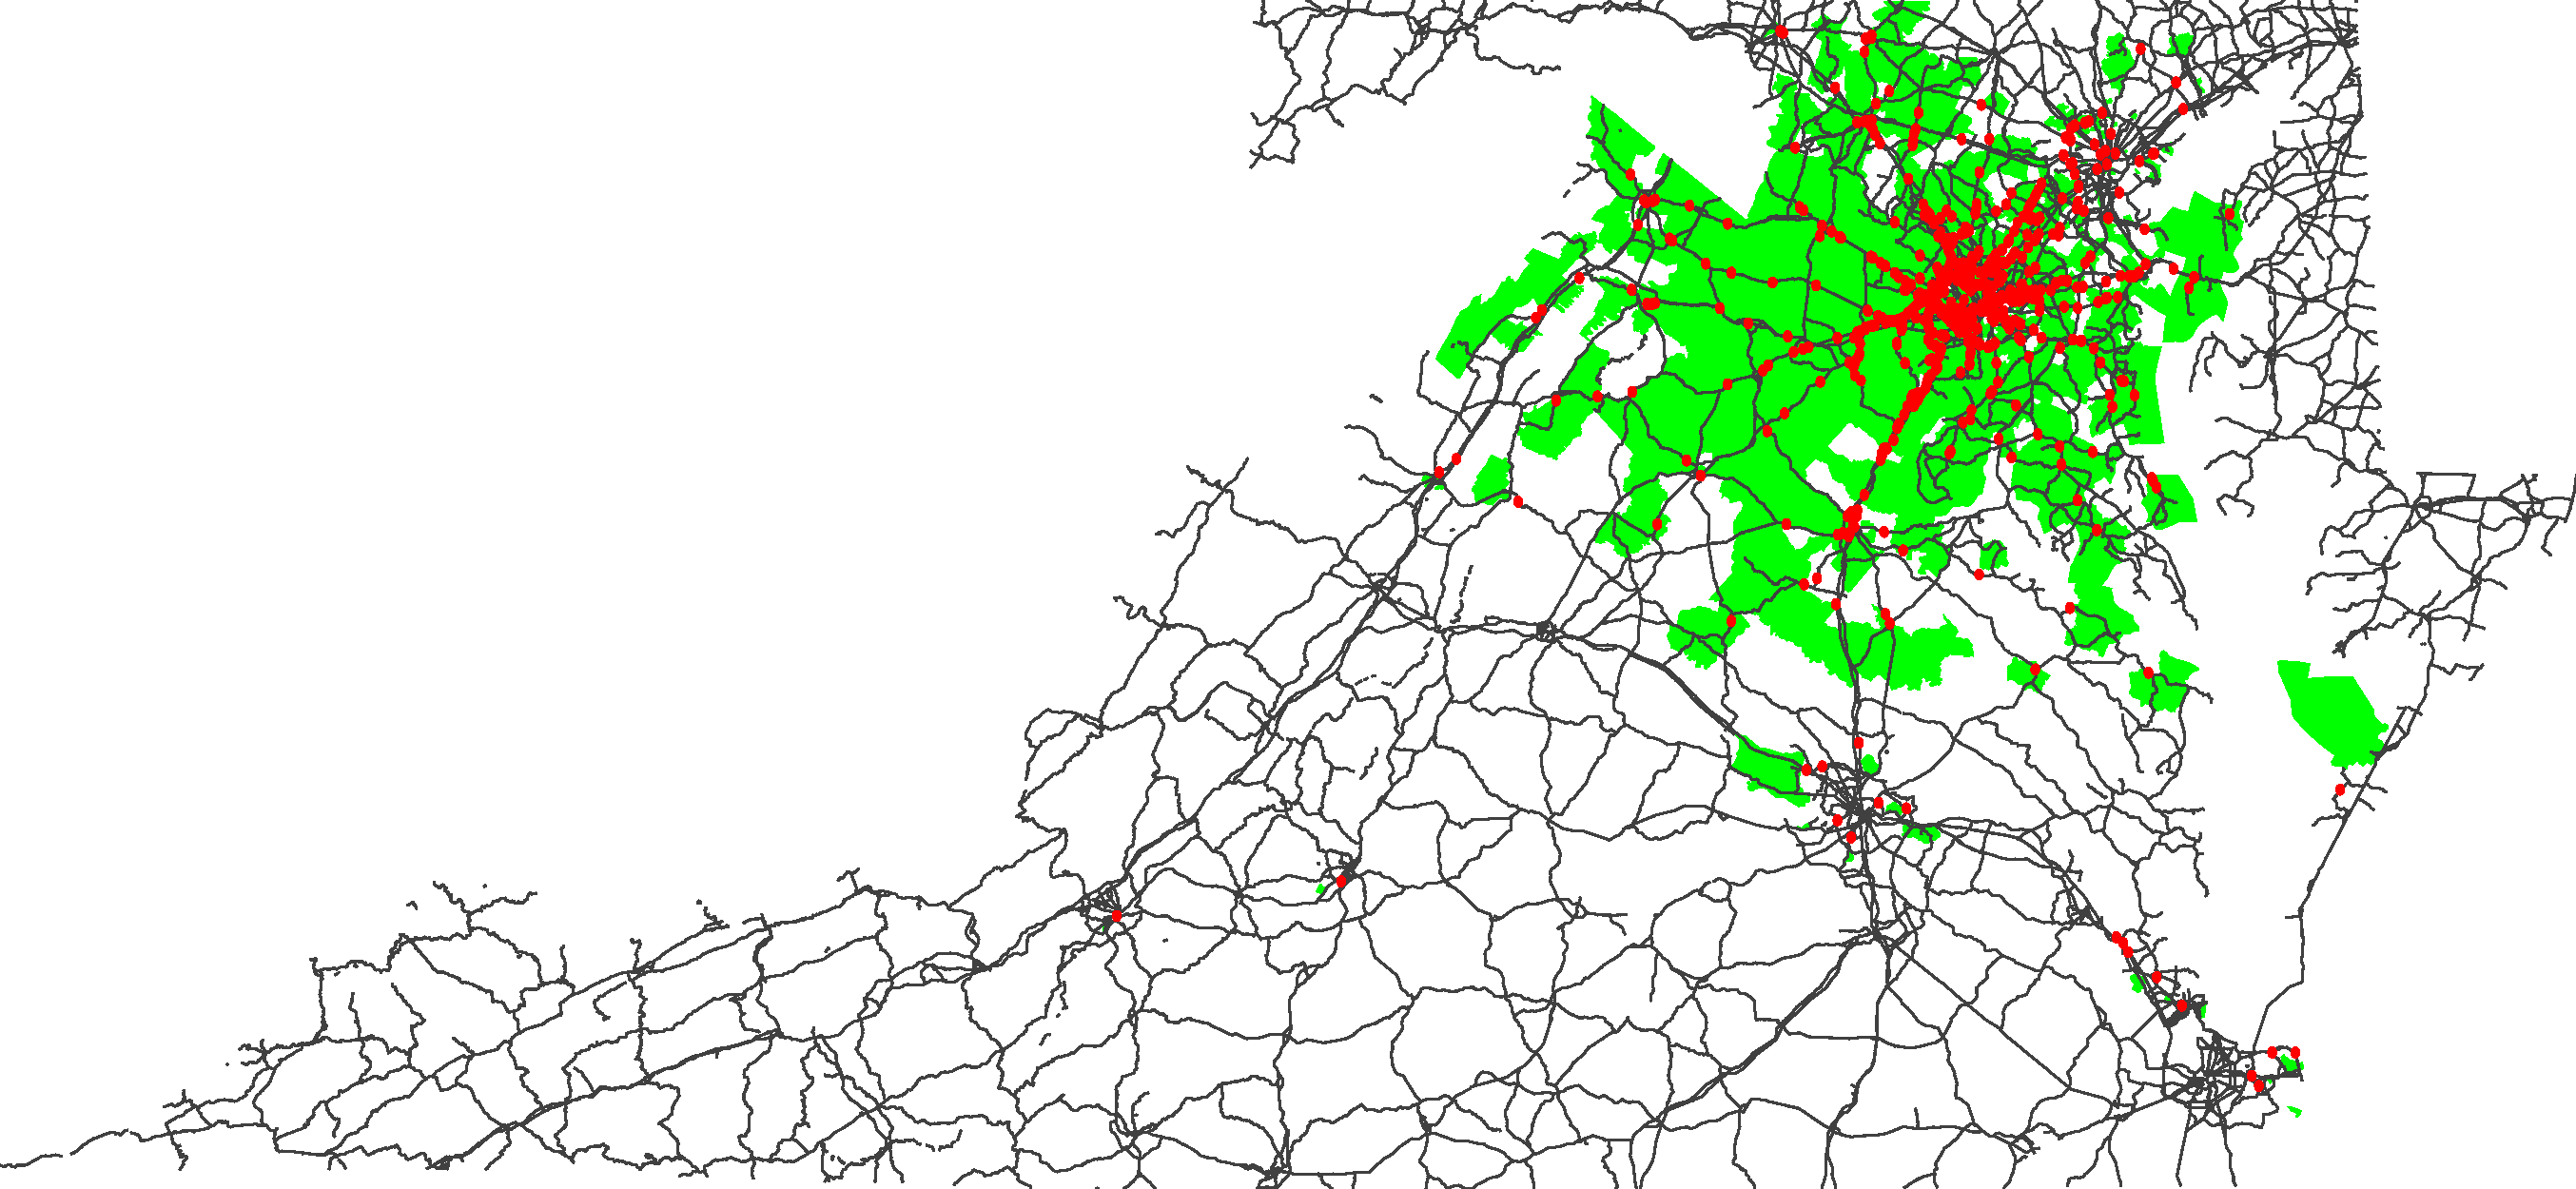
\includegraphics[width=0.45\textwidth]{gridlocknormal.pdf}
  
\includegraphics[width=0.45\textwidth]{gridlockbroken.pdf}
  \caption{The left subfigure shows proper scaling of the agents; the
    right shows what happens when the default of 1.0 is used.}
  \label{fig:properscalefactor}
\end{figure}

\end{description}


\section{Layers Do Not Align}
\label{sec:NonAlignedLayers}

\begin{description}
\item[Problem]~\\
The data between layers does not match.

\item[Solution]~\\
You probably did not align the minimum bonding rectangles between all
the \class{GeomField} layers as directed by recipe \ref{sub:multiplevectorlayers}.

% \begin{Verbatim}[frame=lines,framesep=5mm,commandchars=+\[\]]
% foo
% \end{Verbatim}

\item[Discussion]~\\
Fig. \ref{fig:colorworldMBR} shows what happens when the minimum
bounding rectangles (MBR) between layers are not synchronized. Both figures
show the GeoMason Campus World demo.  The one on the left shows the
demo with the MBRs properly synchronized.  The figure on the right
shows the same demo, but this time all the code that is responsible
for synchronizing the MBRs has been removed.  Note that the buildings
are no longer inside the roads and that the agents are not even
visible. More specifically, given that the underlying coordinate reference system for
this demo is UTM, the units are in meters.  The unmodified building MBR is a
rectangle with defining corner coordinates (1182163, 6986772),
(1182361, 6988786) and the corresponding default agent MBR is (10,
10), (10, 10), which would explain why the agents are not visible.
\begin{figure}[ht]
  \centering
  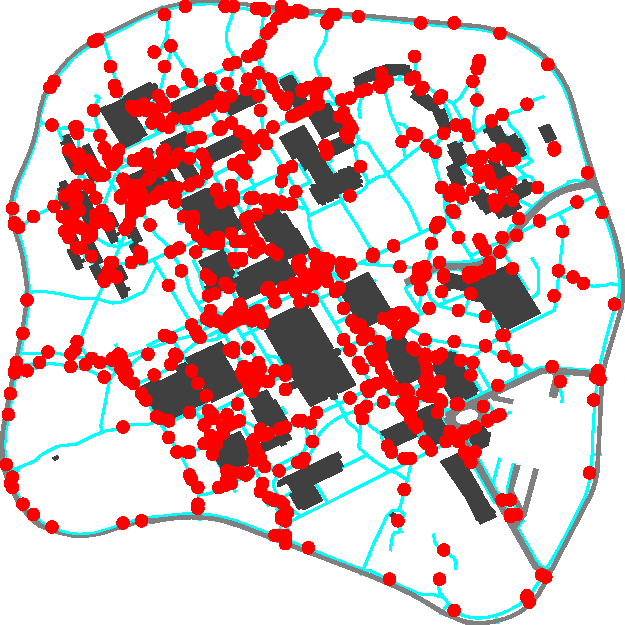
\includegraphics[width=0.45\textwidth]{campusworldnormal.pdf}
  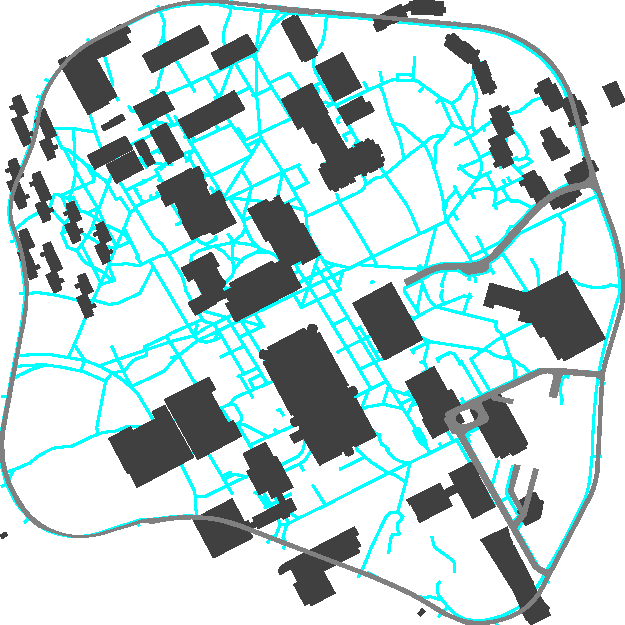
\includegraphics[width=0.45\textwidth]{campusworldbroken.pdf}
  \caption{Shows proper MBR
    alignment on the left, and on the right what happens when the MBRs are not set
    at all}
  \label{fig:colorworldMBR}
\end{figure}

\end{description}


%%
%%
%%
\cleardoublepage % especially in a document where chapters start at right-hand pages
%\phantomsection % for an anchor if you use hyperref
\addcontentsline{toc}{chapter}{Acknowledgements} % if you wish to have a TOC entry
\chapter*{Acknowledgements} % for the actuall unnumbered heading
\thispagestyle{empty} % or plain etc.
\markboth{Acknowledgements}{Acknowledgements} % relevant depending on page style

Thanks to the support of the Office of Naval Research (ONR) under a
Multidisciplinary University Research Initiative (MURI) Grant
No. N00014-08-1-0921, the Joint Improvised Explosive Device Defeat
Office (JIEDDO) J-9 Division and the Office of Naval Research (ONR)
under Government Contract number N00014-09-C-0419, and also NSF grant
0916870 for supporting this work. I would also like to thank the
entire MASON development team and the GMU Center for Social Complexity
without whom this work would not have been possible.  I also would
like to give thanks to Andrew Crooks for valuable feedback and for
providing most of the GeoMason demos that originated as student class
projects from his classes.  I would also like to thank Martin Davis
for writing JTS Topology Suite and for providing valuable help and
feedback in its use.  And, finally, I would like to thank Keith
Sullivan for his contribution to GeoMason; he did yeoman service in
writing the initial incarnations of the native GeoMason shape file
reader and writer classes as well as getting GeoMason portrayals up to
speed.

%%
%%
%%

\cleardoublepage
\footnotesize
\addcontentsline{toc}{chapter}{Index}
\printindex

\end{document}















